%%%%%%%%%%%%%%%%%%%%%%%%%%%%%%%%%%%%%%%%%%%%%%%%%%%%%%%%%%%%%%%%%%%%%%%%%%%%%%%%
% Template for USENIX papers.
%
% History:
%
% - TEMPLATE for Usenix papers, specifically to meet requirements of
%   USENIX '05. originally a template for producing IEEE-format
%   articles using LaTeX. written by Matthew Ward, CS Department,
%   Worcester Polytechnic Institute. adapted by David Beazley for his
%   excellent SWIG paper in Proceedings, Tcl 96. turned into a
%   smartass generic template by De Clarke, with thanks to both the
%   above pioneers. Use at your own risk. Complaints to /dev/null.
%   Make it two column with no page numbering, default is 10 point.
%
% - Munged by Fred Douglis <douglis@research.att.com> 10/97 to
%   separate the .sty file from the LaTeX source template, so that
%   people can more easily include the .sty file into an existing
%   document. Also changed to more closely follow the style guidelines
%   as represented by the Word sample file.
%
% - Note that since 2010, USENIX does not require endnotes. If you
%   want foot of page notes, don't include the endnotes package in the
%   usepackage command, below.
% - This version uses the latex2e styles, not the very ancient 2.09
%   stuff.
%
% - Updated July 2018: Text block size changed from 6.5" to 7"
%
% - Updated Dec 2018 for ATC'19:
%
%   * Revised text to pass HotCRP's auto-formatting check, with
%     hotcrp.settings.submission_form.body_font_size=10pt, and
%     hotcrp.settings.submission_form.line_height=12pt
%
%   * Switched from \endnote-s to \footnote-s to match Usenix's policy.
%
%   * \section* => \begin{abstract} ... \end{abstract}
%
%   * Make template self-contained in terms of bibtex entires, to allow
%     this file to be compiled. (And changing refs style to 'plain'.)
%
%   * Make template self-contained in terms of figures, to
%     allow this file to be compiled. 
%
%   * Added packages for hyperref, embedding fonts, and improving
%     appearance.
%   
%   * Removed outdated text.
%
%%%%%%%%%%%%%%%%%%%%%%%%%%%%%%%%%%%%%%%%%%%%%%%%%%%%%%%%%%%%%%%%%%%%%%%%%%%%%%%%

\documentclass[letterpaper,twocolumn,10pt]{article}
\usepackage{usenix2019_v3}

% to be able to draw some self-contained figs
\usepackage{tikz}
\usepackage{amsmath}
\usepackage{xspace}
\usepackage{url}
\usepackage[most]{tcolorbox}

% added by gaowei 
\usepackage{listings}

\usepackage{xcolor}
\usepackage{caption}

\definecolor{codegreen}{rgb}{0,0.6,0}
\definecolor{codegray}{rgb}{0.5,0.5,0.5}
\definecolor{codepurple}{rgb}{0.58,0,0.82}
\definecolor{backcolour}{rgb}{0.98,0.98,0.98}

\lstdefinestyle{mystyle}{
    backgroundcolor=\color{backcolour},   
    commentstyle=\color{codegreen},
    keywordstyle=\color{magenta},
    numberstyle=\tiny\color{codegray},
    stringstyle=\color{codepurple},
    basicstyle=\ttfamily\footnotesize,
    breakatwhitespace=false,         
    breaklines=true,                 
    captionpos=b,                    
    keepspaces=true,                 
    numbers=left,                    
    numbersep=5pt,                  
    showspaces=false,                
    showstringspaces=false,
    showtabs=false,                  
    tabsize=2,
    language=Python
}

\lstset{style=mystyle}

\usepackage{hyperref}
\usepackage{balance}
\usepackage[normalem]{ulem}
\usepackage{graphicx}
\usepackage{algorithm}
\usepackage{algpseudocode}
\usepackage{amsthm}
\usepackage{amsmath}
\usepackage{multirow}
\usepackage{url}
\usepackage{subcaption}
\usepackage{enumitem}
\usepackage{makecell}
\usepackage{booktabs} 
\usepackage{soul}
\usepackage{textcomp}
\usepackage{pifont}
\usepackage[T1]{fontenc}
\usepackage{inconsolata}
\usepackage{adjustbox}
\usepackage{wrapfig}



\let\Bbbk\relax
\usepackage{amssymb}
\usepackage{bbm}
\usepackage{tabularx}
\usepackage{bbding}

\usepackage[normalem]{ulem}

\newtheorem{theorem}{Theorem}
\newtheorem{lemma}{Lemma}
\newtheorem{remark}{Proposition}

\newcommand{\Prefix}{\textsc{Prompt}}
\newcommand{\gaowei}[1]{\textcolor{orange}{#1}}
\newcommand{\yuheng}[1]{\textcolor{blue}{#1}}
\usepackage[most]{tcolorbox}

\usepackage{tikz}
\newcommand\encircle[1]{\tikz[baseline=(X.base)] 
    \node (X) [draw, shape=circle, inner sep=0pt, fill=black, text=white] {\strut #1};}

\newcommand\wcircle[1]{\raisebox{-0.5ex}{\Large\ding{\numexpr171+#1}}}

% \usepackage[table,xcdraw]{xcolor}

% to avoid warning
% \microtypecontext{spacing=nonfrench}

\newcommand{\cmark}{\ding{51}}%
\newcommand{\xmark}{\ding{55}}%


\theoremstyle{definition}


\newenvironment{denseitemize}{
	\begin{itemize}[topsep=2pt, partopsep=0pt, leftmargin=1.5em] %label=$\star$
		\setlength{\itemsep}{3pt}
		\setlength{\parskip}{0pt}
		\setlength{\parsep}{0pt}
	}{\end{itemize}}


\newcommand{\PHB}[1]{\noindent\textbf{#1}}
\newcommand{\PHM}[1]{\vspace{.4em}\noindent\textbf{#1}} 
 
\newcommand{\SystemName}{\textsc{RollArt}\xspace}

\newcommand{\gw}[1]{\textcolor{blue}{#1}}

\begin{document}

\date{}

% make title bold and 14 pt font (Latex default is non-bold, 16 pt)
% \title{\Large \bf \SystemName: Disaggregated Multi-Task Agentic RL Training at Scale}

 \title{\Large \bf \SystemName: Scaling Agentic RL Training via Disaggregated Infrastructure}
 
\author{
    {\rm Wei Gao$^{\dagger*}$, Yuheng Zhao$^{\dagger*}$, Tianyuan Wu$^{\dagger*}$, Shaopan Xiong$^{\ddagger*}$, Weixun Wang$^{\ddagger*}$, Dakai An$^{\dagger}$,} \\
    {\rm Lunxi Cao$^{\dagger}$, Dilxat Muhtar$^{\ddagger}$, Zichen Liu$^{\ddagger}$, Haizhou Zhao$^{\ddagger}$, Ju Huang$^{\ddagger}$, Siran Yang$^{\ddagger}$,} \\
    {\rm Yongbin Li$^{\P}$, Wenbo Su$^{\ddagger}$, Jiamang Wang$^{\ddagger}$, Lin Qu$^{\ddagger}$, Bo Zheng$^{\ddagger}$, Wei Wang$^{\dagger}$}
    \bigskip \\
    {\em $^{\dagger}$HKUST \quad $^{\ddagger}$Alibaba Group \quad $^{\P}$Tongyi Lab, Alibaba}
    \vspace{0.5cm}
}





% %for single author (just remove % characters)
% \author{
% {\rm Your N.\ Here}\\
% Your Institution
% \and
% {\rm Second Name}\\
% Second Institution
% % copy the following lines to add more authors
% % \and
% % {\rm Name}\\
% %Name Institution
% } % end author

\maketitle
\def\thefootnote{*}\footnotetext{Wei Gao, Yuheng Zhao, Tianyuan Wu, Shaopan Xiong, and Weixun Wang contributed equally to this work.}

\setlength{\floatsep}{3pt plus 2pt minus 1pt}
\setlength{\textfloatsep}{3pt plus 2pt minus 1pt}
\setlength{\intextsep}{3pt plus 2pt minus 1pt}
\setlength{\abovecaptionskip}{3pt plus 2pt minus 2pt}
\setlength{\belowcaptionskip}{3pt plus 2pt minus 2pt}
\setlength{\abovedisplayskip}{3pt plus 2pt minus 2pt}
\setlength{\belowdisplayskip}{3pt plus 2pt minus 2pt}


%!TEX root=../main.tex
\begin{abstract}
Agentic Reinforcement Learning (RL) enables Large Language Models (LLMs) to
perform autonomous decision-making and long-term planning. Unlike standard LLM
post-training, agentic RL workloads are highly \emph{heterogeneous}, combining
compute-intensive prefill phases, bandwidth-bound decoding, and stateful,
CPU-heavy environment simulations. We argue that efficient agentic RL training
requires \emph{disaggregated infrastructure} to leverage specialized, best-fit hardware.
However, naive disaggregation introduces substantial synchronization overhead
and resource underutilization due to the complex dependencies between stages.

We present \SystemName{}, a distributed system designed to maximize throughput for multi-task agentic RL on disaggregated infrastructure. \SystemName{} is built on three core principles: (1) \emph{hardware-affinity workload mapping}, which routes compute-bound and bandwidth-bound tasks to best-fit GPU devices, (2) \emph{fine-grained asynchrony}, which manages execution at the trajectory level to mitigate resource bubbles, and (3) \emph{statefulness-aware computation}, which offloads stateless components (e.g., reward models) to serverless infrastructure for elastic scaling. Our results demonstrate that \SystemName{} effectively improves training throughput and achieves 1.35-2.05\(\times\) end-to-end training time reduction compared to monolithic and synchronous baselines. We also evaluate \SystemName{} by training a hundreds‑of‑billions‑parameter MoE model for Qoder product on an Alibaba cluster with more than 3,000 GPUs, further demonstrating \SystemName{}’s scalability and robustness. The code is available at \url{https://github.com/alibaba/ROLL}.



% Our results demonstrate that \SystemName{} effectively mitigates 
% environment stragglers and achieves significant improvements in training throughput and resource utilization compared to monolithic and synchronous baselines.

% The agentic Reinforcement Learning (RL) emerges as a pivotal technique to enable Large Language Models (LLMs) from passive response to autonomous decision-making and adaptive long-term planning, empowering AI to handle complex and dynamic tasks across domains. RL researchers explore scaling laws in agentic environments and endow LLMs with agentic capability, urging an efficient multi-task agentic RL training system. We assert that efficient multi-task agentic RL necessitates running on disaggregated clusters to leverage specialized hardware. This approach, however, introduces substantial synchronization overhead between stages and can lead to resource underutilization. To address these challenges and fully harness the benefits of disaggregation, we propose \SystemName{}, a system built on three core design principles: (1) map workloads based on hardware affinity; (2) manage execution with fine-grained asynchrony; and (3) characterize computation by statefulness. \SystemName{}’s programming and computation model, as well as its architecture, are designed around these principles. We share using \SystemName{} to train a hundreds‑of‑billions‑parameter MoE model for Qoder product on an Alibaba cluster with more than 3,000 GPUs, and extensive experiments further demonstrate the effectiveness of \SystemName{}.
\end{abstract}


% We also report our experience using \SystemName{} to train a 480B‑A35 Qwen-Coder on an Alibaba cluster with 3{,}072 GPUs, and our extensive empirical analysis demonstrates the effectiveness of \SystemName{}.

%!TEX root=../main.tex
\section{Introduction}
\label{sec:introduction}

Reinforcement Learning (RL) has become a cornerstone for advancing Large
Language Models (LLMs) from passive logical reasoning toward autonomous
decision-making and long-horizon planning~\cite
{deepseekr1,seed-thinking,openaio4}. This paradigm, known as \emph{agentic RL},
requires LLMs to operate effectively within complex, dynamic environments,
ranging from tool use~\cite
{hao2025exploringsuperiorfunctioncalls,wu2025agenticreasoningstreamlinedframework}
to web navigation~\cite
{song2025r1searcherincentivizingsearchcapability,jin2025searchr1trainingllmsreason,jiang2025deepretrievalhackingrealsearch}
and general computer control~\cite
{luo2025guir1generalistr1style,lu2025uir1enhancingefficientaction,liu2025infigui}.
Unlike traditional LLM post-training, agentic RL emphasizes learning through
extensive practice: the agent actively interacts with external environments
to generate \emph{long, multi-turn trajectories}, thereby solving complex reasoning
tasks through trial and error.


The agentic RL training pipeline operates as an iterative cycle comprising
three stages: \emph{rollout}, \emph{reward}, and \emph{training}. During rollout, the agent LLM engages
in a \emph{multi-turn feedback loop} with an environment, generating action tokens
and receiving observations until a termination condition is met, which 
constitutes a \emph{trajectory}. These trajectories
are then evaluated in the reward stage, often by separate models or code sandboxes, to assign scalar
reward signals. Finally, the training stage consumes these labeled
trajectories to update the agent LLM's weights. These updated parameters are then
synchronized back to the rollout workers for the subsequent iteration,
creating a loop of data generation and policy update.



As research institutes investigate \emph{Scaling Laws for Agentic RL}~\cite
{kimiteam2025kimik2openagentic,deepseek_v3_2_speciale}, a fundamental
infrastructure challenge emerges: the resource requirements across the
pipeline are highly \emph{heterogeneous} and often \emph{conflicting}. 
The \textbf{rollout stage}
alone presents a complex composite workload. LLM generation alternates
between TFLOPS-hungry prefill phases---best served by compute-optimized
hardware (e.g., NVIDIA H800)---and bandwidth-bound decoding phases that benefit
from high memory bandwidth (e.g., H20). The ratio of these phases is dictated
by the task structure: long-horizon tasks like \texttt{FrozenLake}~\cite{frozen_lake} or \texttt{SWE-bench}~\cite{swe-bench} are
prefill-heavy, whereas short-turn tasks like \texttt{GEM-math}/\texttt{GEM-game}~\cite{GEM-github} are decoding-dominant.
Concurrently, the agent LLM must interact with thousands of parallel
environments. These environments are often
\emph{stateful}, \emph{CPU-bound simulations} that introduce severe resource contention if
colocated on GPU nodes. In contrast, the \textbf{reward stage} typically consists of
\emph{stateless, parallelizable} workers running diverse evaluations 
from simple CPU scripts~\cite{he2025deepmath,guo2024deepseekCoder}
to complex GPU-based model judgments~\cite{son2024llmasajudgerewardmodel,zhong2024rlhfuseefficientrlhftraining}. Finally, the \textbf{training stage} demands 
high-end GPUs with fast interconnects to sustain the high TFLOPS required for large-scale parameter optimization.


We contend that a single monolithic cluster cannot efficiently satisfy the
diverse, conflicting resource requirements of multi-task agentic RL training.
While a natural solution is to exploit \emph{disaggregated architectures} that
route stages to \emph{best-fit} hardware, current systems fail to fully
realize this potential. Industry-standard systems such as veRL~\cite
{verl,sheng2025hybridflow}, slime~\cite{slime_github}, and rLLM~\cite
{rLLM} remain bound to monolithic GPU clusters. Newer frameworks like AWorld~\cite{aworld} and
DeepSWE~\cite{deepswe2025} introduce \emph{partial disaggregation} by
offloading environments to Kubernetes~\cite{k8s} clusters. However, they still
colocate the resource-heavy rollout and training stages, leaving the resource
mismatch problem unresolved. Even recent system efforts that decouple
training from rollout, such as StreamRL~\cite{StreamRL}, AsyncFlow~\cite
{asyncflow}, SeamlessFlow~\cite{seamlessflow}, and Laminar~\cite
{Laminar}, adopt a \emph{coarse-grained} approach. These systems largely
overlook the inherent heterogeneity of agentic tasks and environments,
limiting their ability to fully exploit specialized hardware for expedited
rollout.




While disaggregation enables hardware specialization, it introduces severe
orchestration challenges due to \emph{heterogeneous communication patterns}
and \emph{synchronization overheads}. First, the data transfer requirements
are highly \emph{unbalanced}. Weight synchronization between training and
rollout clusters is bandwidth-intensive, involving bulk data transfer of hundreds of 
gigabytes and
incurring latency on the order of tens of seconds. Conversely, trajectory
transfers between the agent LLM and environments are smaller (kilobytes to
gigabytes) but suffer from extreme variance: environment instability can
introduce \emph{long-tail latencies} reaching hundreds of seconds (\autoref
{fig:env_time_cdf}), severely blocking dependent stages. Second, in
synchronous training, these communication delays create ``resource bubbles''
(\autoref{fig:paradigm-all-in-one}-Left), where expensive training GPUs idle
while waiting for straggling environments or weight updates. While one could
attempt stitching together current
disaggregated RL frameworks~\cite{StreamRL,seamlessflow,asyncflow} with
Kubernetes-orchestrated agentic environments, such ad-hoc integration 
can only serve for a single job with dedicated, high-bandwidth networks and
does not scale to production-grade, multi-tenant clusters where cross-cluster
links often exhibit dynamic, heterogeneous bandwidth.


To address the aforementioned challenges, we present \SystemName{}, a distributed system
designed to maximize throughput for multi-task agentic RL on disaggregated
infrastructure. \SystemName{} evolves from our prior technical reports on ROLL~\cite{roll} and ROLL-Flash~\cite{rollflash}. Unlike systems that treat the cluster as a uniform
pool, \SystemName{} orchestrates the RL pipeline according to three
core design principles. \textbf{(1) Hardware-Affinity Workload
Mapping:} \SystemName{} allows users to bind an entire stage to a dedicated
hardware resource pool (e.g., constraining training to compute-optimized
GPUs). It also supports \emph{fine-grained affinities} within a stage. This
allows, for example, routing prefill-heavy, compute-bound tasks (e.g., \texttt
{FrozenLake} and \texttt{SWE-bench}) to H800 GPUs while scheduling
decoding-dominant, bandwidth-bound tasks (e.g., \texttt{GEM-math}) on H20
GPUs. The hardware affinity can fully exploit available resources and
maximize the system throughput. \textbf{(2) Fine-grained Asynchrony:} Within rollout, this principle advocates operating
at the \emph{trajectory level} rather than the batch level. By interleaving
environment interaction, LLM generation, and reward computation, the system
effectively masks inter-cluster communication latency and prevents slower
environment stragglers from stalling the entire pipeline. For asynchronous
training, it requires fine-grained control of the asynchrony between rollout
and training to balance gradient stability and system throughput. \textbf{
(3) Statefulness-aware Computation:} To optimize resource
efficiency, \SystemName{} explicitly categorizes components by their state
requirements. It offloads inherently stateless components, such as reward
models, to serverless infrastructure (e.g., Function Compute~\cite
{alibaba_function_compute}), granting the system zero-overhead autoscaling,
multi-tenancy, and fault tolerance without dedicated, hot-standby GPUs.

We realize these principles in \SystemName{}, a distributed system that
combines a declarative programming model with a heterogeneity-aware runtime.
Through Python-based decorators, users explicitly define \emph
{hardware affinities} for specific sub-tasks and register stateless
components to external serverless interfaces. Under the hood, \SystemName
{}'s resource manager allocates heterogeneous resources to specialized \emph
{workers}, while the distributed runtime orchestrates an asynchronous,
trajectory-level workflow. To maximize hardware efficiency, the runtime
integrates optimized execution engines, using inference engines~\cite{vllm, sglang,rtp-llm} for
high-throughput generation and training engine~\cite{shoeybi2019megatron} for
distributed training. The runtime also exposes multiple transfer channels that exploit the underlying heterogeneous network fabric (NVLink, InfiniBand, Ethernet), optimizing both
the stability-critical trajectory transfer and bandwidth-intensive weight synchronization. %  and the stability-critical
% trajectory transfer. 

We implemented \SystemName{} from scratch in approximately 60k lines of
Python code. We evaluate \SystemName{} by training multiple Qwen models~\cite
{qwen-huggingface} on disaggregated clusters, demonstrating that it achieves
up to a 2.05$\times$ speedup over monolithic and synchronous baselines. To
validate scalability and stability in a production setting, we deploy \SystemName{}
to train a large Mixture-of-Experts (MoE) LLM for Qoder~\cite{qoder} product. This
deployment, running continuously for one week on a cluster of over 3,000
GPUs, confirms \SystemName{}'s ability to sustain high throughput and robust fault
tolerance at scale.

%!TEX root=../main.tex
\section{Background}
\label{sec:background}


\subsection{Agentic RL Training}
\label{subsec:multi-task-agentic}

\PHB{The Training Pipeline.}
The training pipeline for multi-task agentic RL is an iterative loop
comprising three distinct computational stages. The first stage is a \textbf
{rollout} for experience collection. In this stage, the agent LLM
(actor) interacts with parallel \emph{environments} to generate training
data. Unlike standard LLM inference, this process is \emph
{multi-turn} and \emph{stateful}~\cite
{kimiteam2025kimik2openagentic,deepseek_v3_2_speciale}. In each turn, the
agent observes a state, generates an action token sequence, and submits it to
the environment. The environment executes the action (e.g., running code,
clicking a link) and returns feedback. This cycle repeats until a termination
condition is met, producing a sequence of state-action pairs known as a \emph
{trajectory}. Once a trajectory is complete, the system proceeds to
a \textbf{reward stage}, where a \emph{reward worker} evaluates the quality
of the agent's actions. This evaluation yields a scalar reward signal,
computed via methods ranging from lightweight rule-based checks~\cite
{he2025deepmath} to computationally intensive model-based judgments
(e.g., LLM-as-a-Judge~\cite
{son2024llmasajudgerewardmodel,zhong2024rlhfuseefficientrlhftraining}).
Finally, the collected trajectories and rewards are consumed by the \textbf
{training stage} to update the agent LLM’s weights using RL algorithms
(e.g., PPO~\cite{schulman2017proximal}, GRPO~\cite{shao2024deepseekmath}). For training performance~\cite{areal}, RL researchers typically adopt \textit{synchronous} RL training which requires strict synchronization of the model weights between the rollout and training stage in each step. 



\begin{table}[t]
\centering
\caption{Taxonomy of Adopted Agentic Environments.}
\label{tab:env-taxomy}
% \vspace{-5pt}
\resizebox{0.48\textwidth}{!}{%
\begin{tabular}{ll l c}
\toprule
\textbf{Environment} & \textbf{Task} \textbf{Domain}   & \textbf{Modality}     & \textbf{\#Turns} \\
\midrule
SWE-bench~\cite{swe-bench}   & SWE           & Text         & 30--50      \\
WebShop~\cite{webshop}     & Web           & Text         & 5--30      \\
FrozenLake~\cite{frozen_lake}  & Game          & Text, Visual & 20--100      \\
GEM-math~\cite{GEM-github}    & Math+Tool Use & Text       & $<5$         \\
GEM-game~\cite{GEM-github}    & Game          & Text         & 1            \\
\bottomrule
\end{tabular}}
\end{table}

\begin{figure}[tb]
    \centering      
    \begin{subfigure}{0.48\textwidth}
        \centering
        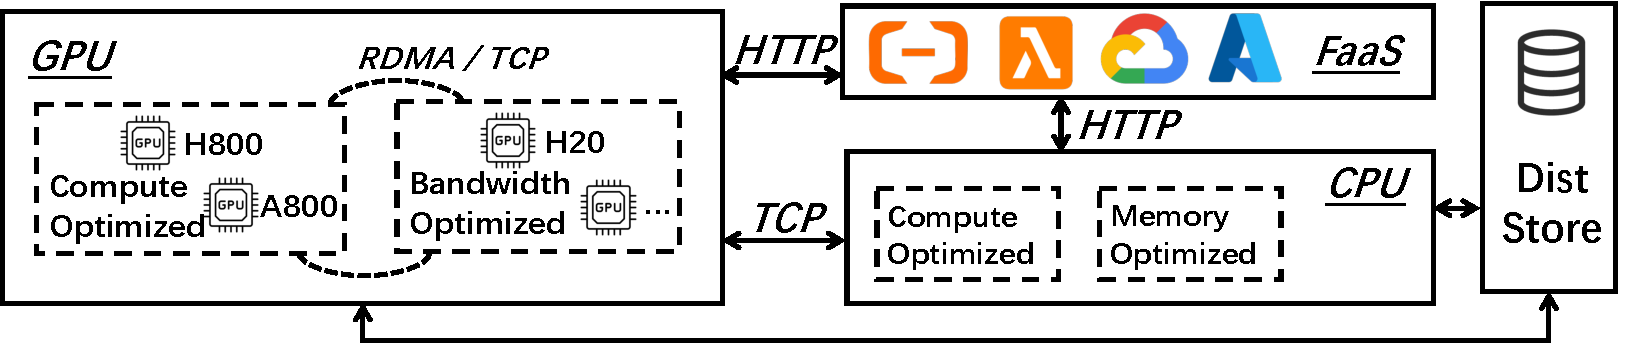
\includegraphics[width=\linewidth]{figs/overview/disaggregated_cluster.pdf}
    \end{subfigure}    
    % \vspace{-5pt}
    \caption{
        Disaggregated infrastructure for agentic RL training.
    }
    \label{fig:disaggregated_cluster}
\end{figure}





\PHM{Environment Heterogeneity}
% \label{subsec:taxonomy-of-env}
A key challenge in agentic RL is the extreme diversity of the environments,
which dictates the system's compute profile. As summarized in \autoref
{tab:env-taxomy}, agentic tasks vary significantly in modality and
interaction frequency. Complex reasoning tasks like \texttt{SWE-bench}~\cite
{swe-bench} (software engineering), \texttt{FrozenLake}~\cite{frozen_lake}
(visual games), and \texttt{WebShop}~\cite{webshop} (eCommerce) require long
interaction horizons (up to 30--100 turns). Frequent interactions force the
agent LLM to repeatedly process the growing context history, making the
workload prefill-heavy and computationally intensive. Conversely, tasks
like \texttt{GEM-Math} and \texttt{GEM‑Game}~\cite{GEM-github} may involve
fewer turns (up to five) but require generating longer chains of
thought per action. These workloads are decoding-heavy, shifting the
bottleneck from compute to memory bandwidth. This variance means that 
the infrastructure must adapt to the specific characteristics of the current task's rollout.











\subsection{Disaggregated Cluster Infrastructure}
\label{subsec:disaggregated-cluster}

\PHB{The Case for Disaggregation.} 
The extreme heterogeneity of agentic RL workloads, ranging from
compute-intensive training to stateful environment simulation (\S\ref
{subsec:multi-task-agentic}), renders monolithic architectures inefficient.
Consequently, agentic RL training must transition to a \emph
{disaggregated infrastructure} that decouples these demand-conflicting
computation stages into specialized resource pools. As illustrated
in \autoref{fig:disaggregated_cluster}, in a typical disaggregated
infrastructure, \emph{training clusters} utilize high-end, compute-optimized GPUs 
(e.g., NVIDIA H800) for massive throughput; \emph{inference clusters} 
leverage bandwidth-optimized hardware (e.g., H20) to serve memory-bound decoding; 
\emph{CPU clusters} provide elastic capacity for diverse, containerized runtime 
environments orchestrated by Kubernetes~\cite{k8s}; and \emph{serverless infrastructure}
handles bursty, stateless workloads like reward evaluation. 
These pools are interconnected via standard network fabrics, relying on distributed storage for persistent logging and fault tolerance.



\PHM{Sync. vs. Async. Training.} 
While disaggregation resolves resource mismatches, it introduces non-trivial
orchestration challenges to the training paradigm that dictates 
the trade-off between system throughput
and algorithmic consistency.

\underline{\emph{1) Synchronous Training:}}
This paradigm enforces strict consistency by blocking the rollout stage until the
latest model weights are received from the training cluster. In a
disaggregated setting, however, this introduces substantial ``dependency
bubbles'' (\autoref{fig:paradigm-all-in-one}-Left), where expensive GPUs sit \emph{idle}
during the high-latency weight synchronization and straggler-bound
environment steps (\S\ref{sec:motivation}). 

\underline{\emph{2) Asynchronous Training:}}
To mitigate these bubbles, systems can adopt \emph{asynchronous} paradigms
(e.g., one-off RL training~\cite{deepscaler2025} as shown in \autoref
{fig:paradigm-all-in-one}-Right). Here, rollout and training execute \emph{in parallel}: the
training stage consumes trajectories generated by slightly older policies (e.g.,
one iteration behind in one-off training), 
while the rollout stage continuously produces new data. This approach
effectively masks the synchronization latency and straggler effects inherent to
disaggregation, trading a degree of policy freshness (staleness) for
maximized hardware utilization and system throughput.


\begin{table}[t]
\centering
\caption{NVIDIA GPU specifications.}
\label{tab:nvidia-gpu-specs}
% \vspace{-5pt}
\small
\begin{tabular}{lcc}
\toprule
Hardware Specification                & H20            & H800           \\
\midrule
TFLOPS         & 148            & 989.5 \\
HBM capacity        & 96GB  & 80GB           \\
HBM bandwidth       & 4TB/s & 3.35TB/s       \\
NVLink bandwidth    & 900GB/s & 400GB/s      \\
Normalized Cost~\cite{megascale-infer} & 1.00          & 2.85 \\
\bottomrule
\end{tabular}
\end{table}


\begin{figure}[tb]
    \centering      
    \begin{subfigure}{0.48\textwidth}
        \centering
        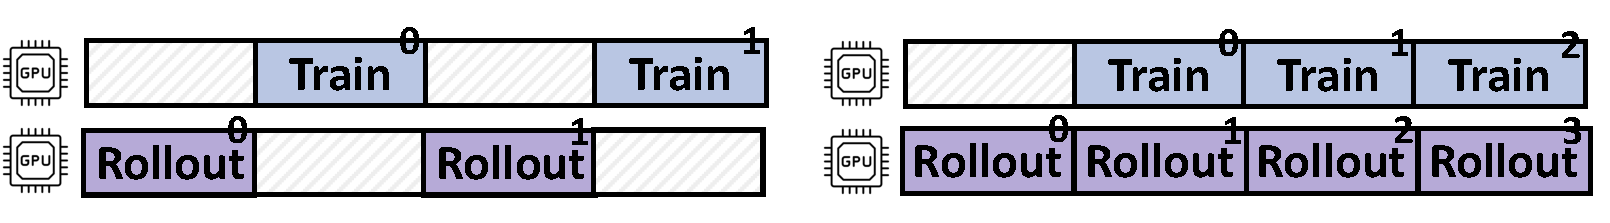
\includegraphics[width=\linewidth]{figs/paradigm/sync_pattern.pdf}
    \end{subfigure}    
    \vspace{-5pt}
    \caption{
        Synchronous vs. asynchronous training.
    }
    \label{fig:paradigm-all-in-one}
\end{figure}


\section{Characterization and System Requirements}
\label{sec:motivation}


To motivate the design of \SystemName{}, we conduct a comprehensive workload
characterization of multi-task agentic RL training. Based on these empirical
observations, we derive a set of critical system requirements (summarized in
the boxes below) that \SystemName{} must satisfy.

\subsection{Stage Computation}
\label{subsec:resource-req-within-stage}

\PHB{Training Step Latency Breakdown.} 
We first profile the end-to-end latency of a standard training iteration to
identify the dominant cost components. We train Qwen3-8B/32K on 32 H800 GPUs
using the \texttt{SWE-bench} environment (batch size 128), where the agent LLM
interacts with a containerized sandbox for software engineering tasks. The
interaction involves two core operations: \texttt{env.reset} for environment
initialization via Docker image pulling and container launching, and \texttt{env.step}
for agent's action execution.


\begin{figure}[t]
    \centering      
    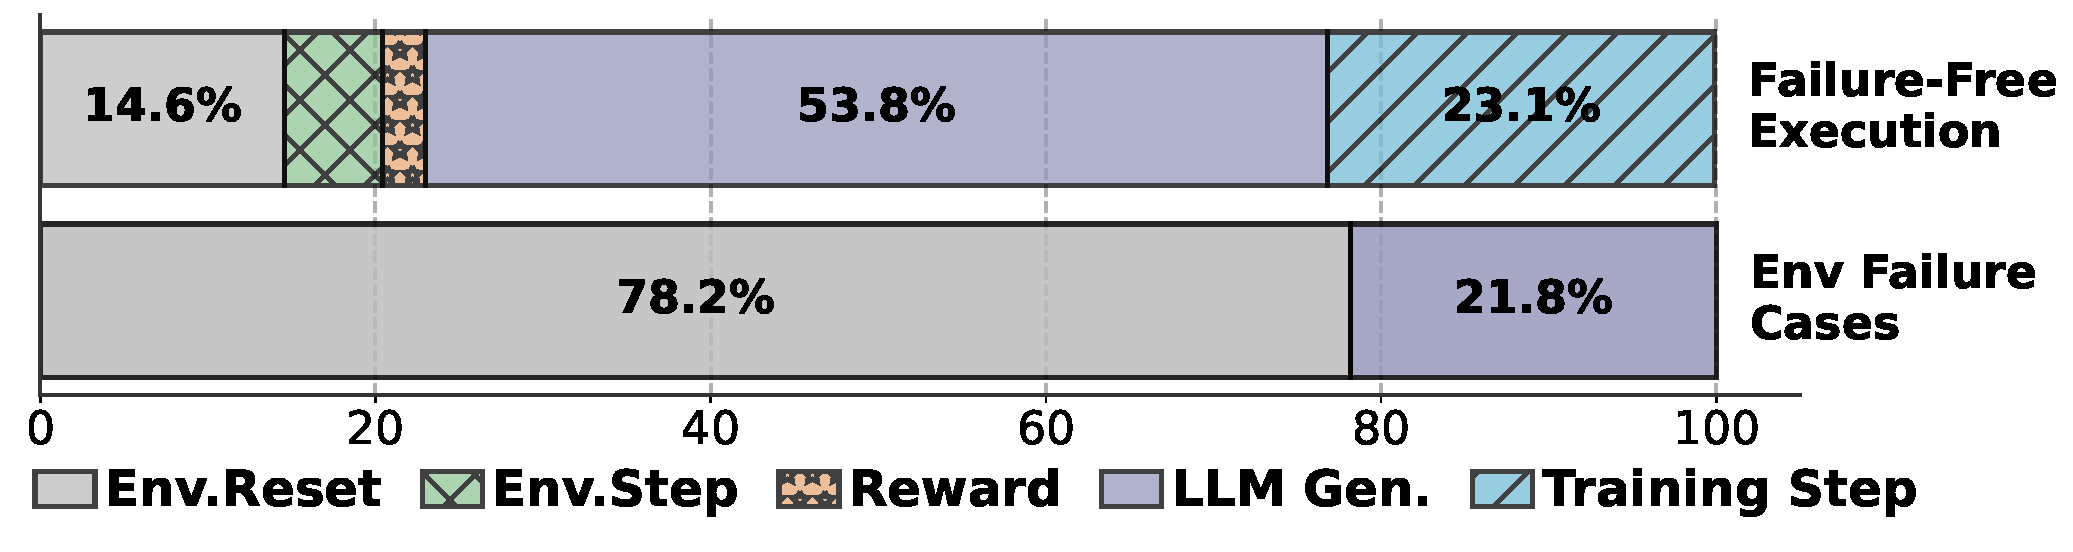
\includegraphics[width=\linewidth]{figs/time/Qwen3-8B-GPU16-sync_time_distribution_fixed.pdf}  
    % \vspace{-8mm}
    \caption{
       Breakdown of a training step: successful runs (top, avg=365.7s) versus execution with environment failures (bottom, avg=513.3s). 
    }
    \label{fig:time_breakdown}
    % \vspace{-5mm}
\end{figure}


\autoref{fig:time_breakdown} breaks down the latency of five \emph
 {successful} iterations against five iterations containing \emph
 {environment failures}. In successful runs, the average iteration time is
 366 seconds, with LLM generation dominating (54\%), followed by training
 (23\%) and environment initialization (15\%). However, in iterations where
 environment timeouts due to failures, the average time spikes to 513
 seconds. Crucially, in these failure scenarios, \texttt{env.reset} alone
 consumes 78\% of the rollout time, shifting the bottleneck entirely from GPU
 computation to environment overhead. Our production data indicates these
 failures are not rare corner cases, occurring approximately once every ten
 iterations. While prior works~\cite{rollpacker,RhymeRL} report that LLM
 generation dominates RL runtime (>80\%), our empirical study reveals that in
 agentic RL, efficient management of the environment lifecycle is the
 paramount challenge.




\begin{figure}[tb]
    \centering
    \begin{subfigure}{0.235\textwidth}
        \centering
        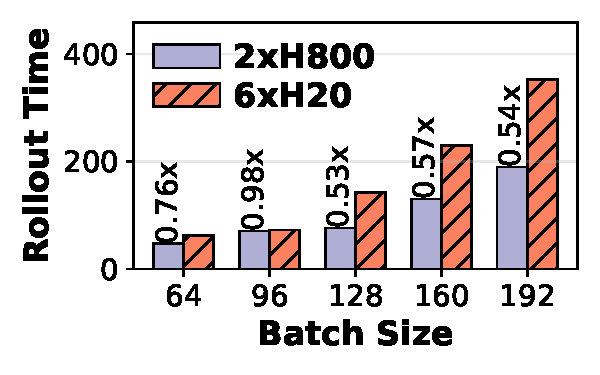
\includegraphics[width=\linewidth]{figs/disagg_motivation/osdi_frozen_lake_decoding_1024_bar.pdf}
        \caption{\texttt{FrozenLake} \small{[Prefill-Heavy]}.}
        \label{fig:prefill-heavy-task}
    \end{subfigure}
    \begin{subfigure}{0.235\textwidth}
        \centering
        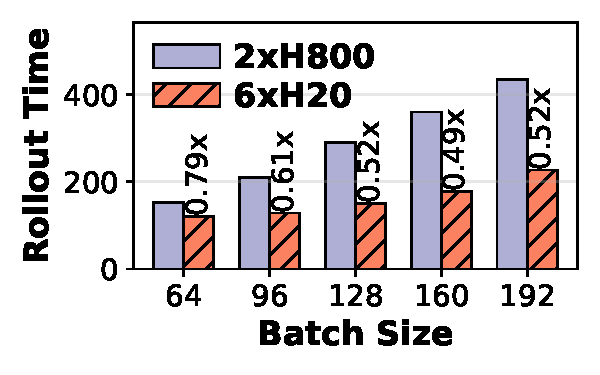
\includegraphics[width=\linewidth]{figs/disagg_motivation/osdi_gem_math_thinking_decoding_4096_bar.pdf}
        \caption{\texttt{GEM-Math} \small{[Decode-Heavy]}.}
        \label{fig:decode-heavy-task}
    \end{subfigure}
    \vspace{-10pt}
    \caption{End-to-end rollout time (seconds) of different tasks on H20 and H800 GPUs across varying batch sizes.}
    % \vspace{-5pt}
    \label{fig:motivation-task-affinity}
\end{figure}


\PHM{Divergent Hardware Affinities in Generation.} 
Modern GPUs expose different trade-offs between compute capability, memory
capacity, and cost (\autoref{tab:nvidia-gpu-specs}). While recent RL
systems~\cite{StreamRL,asyncflow,seamlessflow} advocate physically decoupling
generation from training---assigning rollout to cost-effective,
bandwidth-optimized GPUs (e.g., NVIDIA H20) and training to
compute-optimized devices (e.g., H800)---our characterization reveals that \emph{this
static assignment is insufficient for agentic workloads}. LLM generation
comprises two distinct phases with opposing resource demands: the 
compute-bound prefill phase and the memory-bandwidth-bound decoding phase. In
environments with a few interaction turns and reasoning thinking pattern,
most of the runtime is spent in decoding (decoding-heavy); conversely, in
environments with many turns, the prefill phase dominates and demands high
compute throughput (prefill-heavy). In our production clusters,
agentic RL tasks exhibit a clear \emph{bimodal distribution}, featuring 
either a small number of interaction turns ($< 5$) or a large number ($> 10$).




To quantify this divergence, we run a prefill-heavy task (\texttt
{FrozenLake}) and a decoding-heavy task (\texttt{GEM-Math}) using
Qwen3-8B/32K for ten iterations with prefix caching enabled. For a
cost-equivalent comparison, we execute the workloads on two distinct hardware
configurations: one with 6 H20 GPUs and the other with 2 H800 GPUs. As shown
in \autoref{fig:prefill-heavy-task}, the compute-dense H800 outperforms the
H20 on \texttt{FrozenLake}, reducing end-to-end rollout time to as low as 0.53$\times$. Conversely, for \texttt{GEM-Math} (\autoref{fig:decode-heavy-task}), the
H20's superior memory bandwidth expedites the decoding phase, the H20's higher memory
bandwidth accelerates decoding, reducing rollout time to 0.49$\times$--0.79$\times$
of the H800. These
results invalidate the dogmatic assumption that generation is uniformly
bandwidth-bound. Instead, maximizing throughput requires 
dynamically mapping tasks to their best-fit hardware. 




\begin{tcolorbox}[colback=blue!5!white,colframe=gray!75!black,left=1mm, right=1mm, top=0.5mm, bottom=0.5mm, arc=1mm]
\noindent\textbf{R1:} The optimal resource allocation of LLM generation should align workload characteristics (e.g., prefill- vs. decoding-heavy, batch size) with hardware capabilities.
\end{tcolorbox}



\begin{figure}[tb]
    \centering      
    \begin{subfigure}{0.2\textwidth}
        \centering
        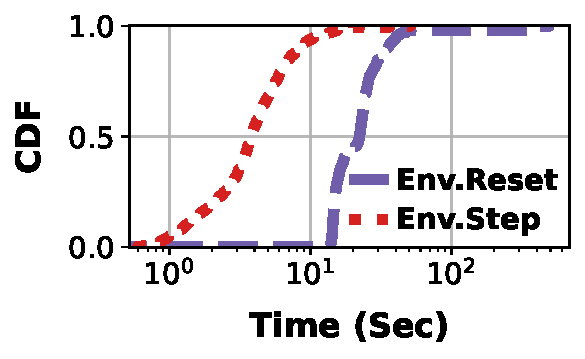
\includegraphics[width=\linewidth]{figs/time/Qwen3-8B-GPU16-sync_time_cdf.pdf}
        \caption{Env Time Distribution.}
        \label{fig:env_time_cdf}
    \end{subfigure}
    \begin{subfigure}{0.27\textwidth}
        \centering
        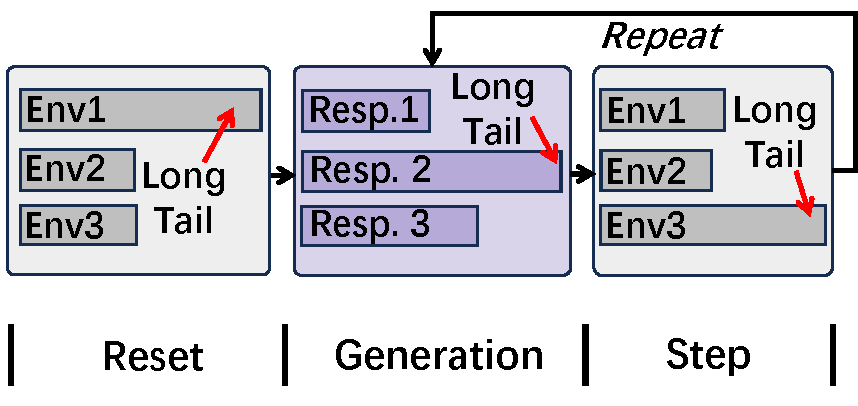
\includegraphics[width=\linewidth]{figs/async_env_illustration/env-long-tail.pdf}
        \caption{Batched Env Interaction.}
        \label{fig:sub-batched_env_interaction}
    \end{subfigure}
    
    % 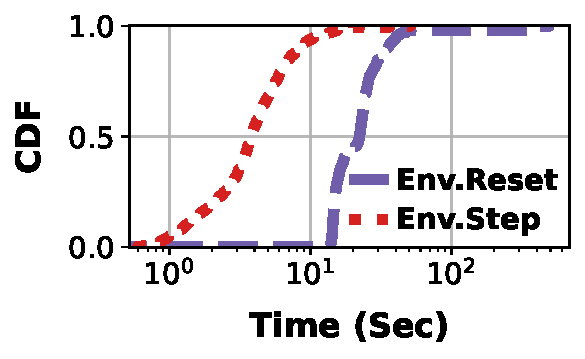
\includegraphics[width=0.48\linewidth]{figs/time/Qwen3-8B-GPU16-sync_time_cdf.pdf}  
    % \vspace{-3mm}
    \caption{The analysis of environment interaction: (a) Cumulative distribution function of time (log-scaled) taken for environment initialization (\texttt{env.reset}) and environment step (\texttt{env.step}). (b) Illustration of how long-tail environments affect multi-turn rollouts under batched env interaction.
    }
    \label{fig:env_analysis}
    % \vspace{-5mm}
\end{figure}

\PHB{Heavy-Tailed Environment Execution.} 
Our production experience running thousands of concurrent environments warrant that resource isolation without interference is essential. Resource sharing can lead to severe issues, such as concurrent disk I/O exhausting shared quotas and causing cascading failures. Consequently, we employ dedicated Kubernetes clusters to manage and isolate each containerized environment.

Substantial prior systems~\cite{rollpacker,StreamRL,RhymeRL} have analyzed the long-tail behavior of LLM generation. \autoref{fig:env_time_cdf} illustrates a similar long-tail distribution in the latency of \texttt{env.reset} and \texttt{env.step} operations, with the effect particularly pronounced for \texttt{env.reset}. In our internal production deployments, the long-tail delay of \texttt{env.reset} can reach hundreds of seconds, mainly due to two factors:
(1) network contention, where hundreds of environment workers simultaneously fetching docker images can saturate network links and overwhelm the image registry service, and (2) compute and I/O contention on host nodes, where launching new containers consumes substantial CPU and disk resources.
% These long-tail environment operations act as stragglers and degrade the rollout efficiency. 


The long-tail environments would become stragglers and delay the end-to-end rollout latency. Specifically, the agent LLM interacts with multiple environments \emph{simultaneously}. Since underlying LLM engines execute requests in batches, it is natural to batch environment interactions with the agent LLM as well. \autoref{fig:sub-batched_env_interaction} illustrates this batched execution pattern, in which the long-tail environment behavior can significantly increase end-to-end rollout latency. Fast environments are forced to wait for the slowest ones before the next generation step can proceed. 
Our profiling (\autoref{fig:time_breakdown}) indicates that batched environment interaction increases rollout time by up to 21.3\% compared to ideal execution, an overhead that compounds as environment failure rates increase. 



\begin{tcolorbox}[colback=blue!5!white,colframe=gray!75!black,left=1mm, right=1mm, top=0.5mm, bottom=0.5mm, arc=1mm]
\textbf{R2:} Environment execution, including \texttt{env.reset} and \texttt{env.step},
is prone to extreme long-tail latency. To prevent stragglers from stalling the pipeline, the system must abandon batched environment interaction in favor of fine-grained, asynchronous environment management.
\end{tcolorbox}

\begin{figure}[tb]
    \centering      
    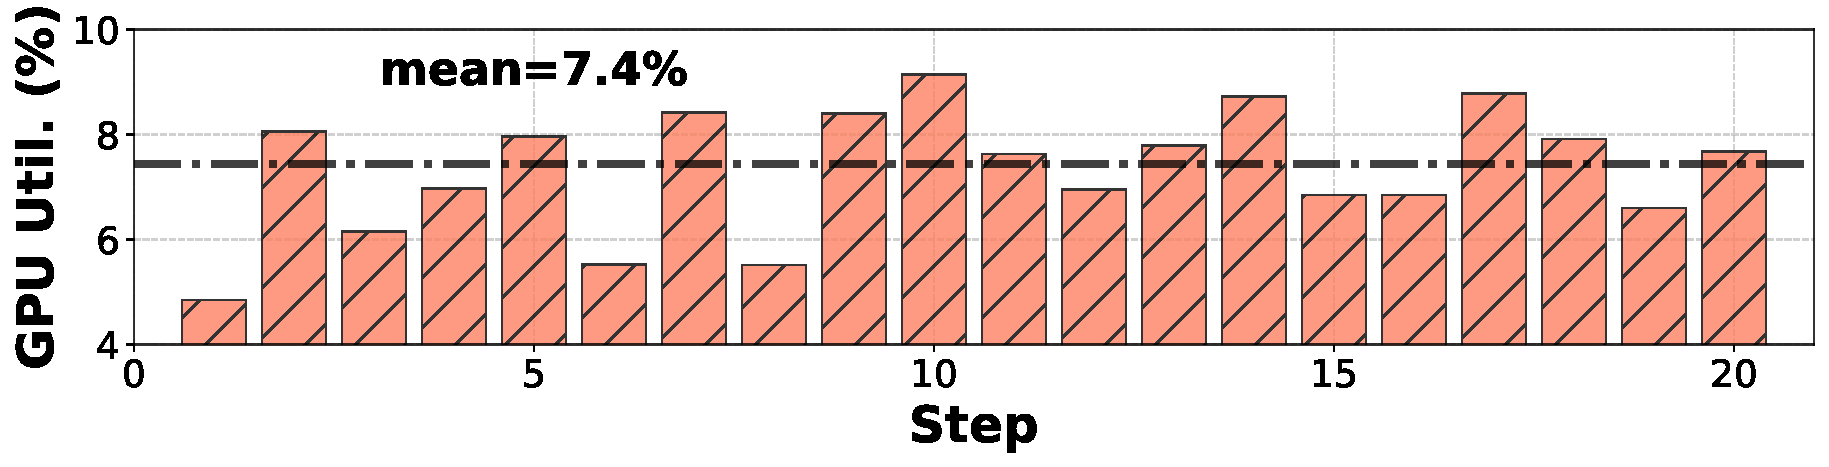
\includegraphics[width=\linewidth]{figs/reward/gpu_utilization_7B.pdf}  
    \vspace{-12pt}
    \caption{
        Inefficient resource usage when dedicating local GPUs for reward computation.
    }
    \label{fig:reward_utilization}
    % \vspace{-10pt}
\end{figure}

\PHB{Stateless Reward Computation.}
The reward stage follows the rollout stage, and most reward computations can be implemented as \emph{stateless functions}. For lightweight code-based and rule-based rewards, the resource demand is relatively small, making it natural to offload these workers on a serverless platform for scalable and low-latency computation. The LLM-based reward computation demands intensive GPUs, contending with rollout workers for GPU resources. A common practice is to reserve dedicated GPUs for reward LLMs. As an example, in our Qwen3-8B/32K \texttt{SWE-bench} experiment with a batch size of 128, we allocate 4 H800 GPUs to a dedicated 7B reward LLM and 28 H800 GPUs to rollouts. However, the reward GPUs achieve only 7.4\% average utilization across steps (\autoref{fig:reward_utilization}). Since the reward LLM’s parameters remain fixed during training, it can be treated as a stateless function, which makes serverless deployment~\cite{Torpor, ServerlessLLM, BLITZSCALE} a promising approach to improving resource utilization.



\begin{tcolorbox}[colback=blue!5!white,colframe=gray!75!black,left=1mm, right=1mm, top=0.5mm, bottom=0.5mm, arc=1mm]
\noindent\textbf{R3:} Reward workers are stateless and typically exhibit low utilization, making them well-suited for serverless deployment to improve overall resource efficiency.
\end{tcolorbox}


\subsection{Inter-Stage Communication}
\label{subsec:communication-between-stage}
% Beyond computation, inter-stage communication is critical for agentic RL training. We next analyze two types of communication: stability-critical, small-packet \emph{trajectory transfer} and bandwidth-sensitive, large-volume \emph{weight transfer}.

Beyond computation, inter-stage communication is a critical role in agentic RL training, comprising two distinct types: stability-critical, small-packet \emph{trajectory transfer} and bandwidth-intensive, large-volume \emph{weight update}.


\begin{table}[t]
\centering
\caption{\small Transmission overhead from the training cluster to the inference cluster over TCP and RDMA.}
\label{tab:llm-transmission}
\scriptsize
\resizebox{0.45\textwidth}{!}{%
\begin{tabular}{lcccc}
\toprule
\textbf{Model} & \textbf{Size (GB)} & \textbf{TCP (s)} & \textbf{RDMA (s)} & \textbf{Speedup} \\
\midrule
Qwen3-8B & 15.26  & 6.911  & 5.466  & 1.264$\times$ \\
Qwen3-14B & 27.51  & 14.437  & 5.817  & 2.482$\times$ \\
Qwen3-32B & 61.02  & 29.649 & 9.442 & 3.140$\times$ \\
\bottomrule
\end{tabular}
} % end resizebox
\end{table}


\PHB{Stability-Critical Trajectory Transfer.} The transmission overhead of trajectory data is small compared with the overall training time. In particular, frequent environment interactions are more likely to become the performance bottleneck due to network latency. In practice, environment interaction should prioritize \emph{network stability} over \emph{network bandwidth}. Asynchronous execution between environment interaction and LLM generation is an effective way to prevent from becoming this bottleneck.


\PHM{Bandwidth-Intensive Weight Update.} 
During training, the agent LLM periodically updates its weights, which must then be synchronized with the rollout stage. This weight synchronization is the dominant source of inter-stage communication overhead. We measure the end-to-end transmission cost of synchronizing model parameters between the training and inference clusters using Mooncake~\cite{qin2024mooncake} over TCP (200 Gbps Ethernet) and RDMA (400 Gbps InfiniBand), and report the results in \autoref{tab:llm-transmission}. RDMA provides higher bandwidth and lower communication overhead than TCP. In \emph{synchronous} RL training, the rollout stage can only proceed after the latest agent LLM weights have been synchronized. As a result, the substantial cost of weight transmission over low-bandwidth links can increase end-to-end training time and diminishes the speedup of disaggregated training (\autoref{fig:paradigm-all-in-one}-Left).

In asynchronous training (\autoref{fig:paradigm-all-in-one}-Right),  the training and rollout stages execute in parallel on separate GPUs. Although this introduces data staleness, many prior works~\cite{rollflash,areal,RhymeRL} empirically observe that asynchronous training can preserve model quality even under a high data staleness. Given the dominant rollout overhead, asynchronous training can effectively hide both training and weight synchronization costs with rollout, thereby reducing end-to-end training latency.


\begin{tcolorbox}[colback=blue!5!white,colframe=gray!75!black,left=1mm, right=1mm, top=0.5mm, bottom=0.5mm, arc=1mm]
\textbf{R4:} Asynchronous RL post-training is desired to improve training efficiency, particularly in disaggregated setups.
\end{tcolorbox}


%!TEX root=../main.tex
\section{Design Principles}
\label{sec:design-principle}
We present our design principles to meet above requirements for multi-task agentic training on disaggregated infrastructure.


\subsection{P1: Hardware-Affinity Workload Mapping}
Our first principle is to map workloads to resources based on their \textit{hardware affinity} to meet requirement \textbf{R1} (highlighted in the box of \S\ref{subsec:resource-req-within-stage}). Users are allowed to define a collection of hardware types at the granularity of both stages and individual trajectories. At the stage level, the training stage can be executed on GPUs, while environment can run on CPUs. At the trajectory level, this principle enables even finer optimization. For example, within the rollout stage, trajectories whose generation is dominated by prefill and does not hit memory limits can be routed to H800 GPUs, whereas trajectories dominated by decoding can be scheduled on H20 GPUs (\S\ref{subsec:resource-req-within-stage}). Similarly, within the reward stage, the reward LLM can run on GPUs, while code‑sandbox execution can run on CPUs. The fine‑grained mapping achieves maximized efficiency.





\subsection{P2: Fine-Grained Asynchronous Execution}
To comply with \textbf{R2} and \textbf{R4}, we introduce our second principle: the diverse communication patterns of disaggregated agentic training can be addressed with fine‑grained asynchrony. Particularly, it should realize the following designs. 

\noindent\textbf{Trajectory-level Rollout Scheduling.} Conventional approaches~\cite{verl} perform LLM generation, environment interaction, and reward computation in a batched manner, which leads to substantial resource wastage and long rollout latency (\S\ref{subsec:communication-between-stage}). In contrast, trajectory-level scheduling creates a continuous pipeline in which LLM generation for one trajectory overlaps with environment interaction for another and reward computation for a third. This pipelined execution reduces resource idleness and hides environment communication delays, improving resilience to environment instability.



\noindent\textbf{Managed Rollout-Train Synchronization.}
Asynchronous RL training decouples the rollout and training stages, allowing them to proceed in parallel. The rollout stage continuously produces trajectories, while the training stage consumes these trajectories and periodically synchronizes updated model weights with the inference workers. Our managed synchronization mechanism exposes explicit control over the rate at which completed trajectories are consumed. 
% (2) the frequency and networking fabric used for model weight synchronization. 
This control allows practitioners to flexibly configure the asynchronous bound (defined in \S\ref{subsec:async-workflow}) to balance the training stability, system throughput, and model weight synchronization overhead. 



\subsection{P3: Statefulness-Aware Computation}
The third principle satisfies \textbf{R3}: we perform statefulness-aware computation. A stateless system component's output depends solely on its input, rendering each execution independent and thus ideal for optimization on a serverless platform.
% This enables employing a serverless platform to optimize it. 

% A stateful component maintains an internal state that persists and evolves across invocations. Differently,


% classify each computational component as either \emph{stateless} or \emph{stateful}.

\noindent\textbf{Rollout: LLM generation.} Production systems typically deploy LLM generation using a serverful architecture to achieve low latency and high throughput. Recently, Tinker~\cite{tml2025tinker} explores elastic serving for RL rollouts, but is designed around LoRA~\cite{hu2021loralowrankadaptationlarge}, whereas full-parameter training is more urgent for production-grade LLMs. 





\noindent\textbf{Rollout: Environment.} This stage is inherently stateful, as the environment (for example, a coding workspace, web browser, or game) is updated by each action. All actions in a trajectory must be routed to the same persistent environment instance, requiring session affinity.


\noindent\textbf{Stateless Reward.} A reward worker takes a trajectory as input and produces a scalar value without retaining any memory of past evaluations. This property makes it well suited to a serverless computation model, enabling shared, multi-tenant \textit{Reward-as-a-Service} that can scale elastically to and from zero, thereby maximizing resource utilization.


\noindent\textbf{Training.} This stage is inherently stateful, necessitating a dedicated GPU cluster. 



\lstset{basicstyle=\scriptsize\ttfamily}
%!TEX root=../main.tex
\section{Programming and Computation Model}
\label{sec:programming-model}
We introduce \SystemName{}, which realizes above design principles via following programming and computation model. 




\begin{figure}[t]
\centering
% \scriptsize
\begin{lstlisting}[
    caption={The declarative programming model of \SystemName{}.
    },
    label={list:api-example-1}
]
import rollart.distributed as rdist
from rdist.worker import AcrtorTrainCls, ActorGenCls, RewardCls
from rdist import ResourceManager as RM

# 1. Single Controller Example
class MyActorTrain(ActorTrainCls):
    @rdist.register(mode="execute_all")
    def compute_gradients(self, input_tensor):
        ...

# 2. Define actor_gen on heterogeneous GPUs
# 2.1 heterogeneous GPU allocation. 
gen_rm=RM( {"H800": list(range(0, 8))},  
           {"H20", list(range(8, 32))})
# 2.2 hardware affinity mapping
class HeteroActorGen(ActorGenCls):
    @rdist.hw_mapping(
    hw_affinity={"FrozenLake": "H800","default": "H20"}
    )
    def generate(self, input_ids:List[int], 
                tag_name:str="default"):
        return self.model.process(prompt)

# 3. Define a serverless reward computation func
class ServerlessRewardWorker(RewardCls):
    @rdist.register_serverless(
        attribute='reward_proxy',
        serverless_url='fc://xxx.xxx')
    def compute_rewards(self, traj: list):
        prompt = f"Evaluate the trajectory:{traj}"
        return ray.get(self.reward_proxy(prompt))

    
\end{lstlisting}
% \vspace{-15pt}
\end{figure}




\subsection{Declarative Programming Model}
In the runtime, a worker is the minimum unit to own resources. \autoref{list:api-example-1} shows the programming model defined at the worker function level, giving the runtime fine-grained visibility into resource usage. The details are as follows.



\noindent\textbf{Single Controller.} This programming model is widely adopted in industrial RL frameworks~\cite{verl,slime_github} as it streamlines the construction of agentic RL pipelines. \SystemName{} adopts this model and realizes it via the \texttt{register} decorator. When the execution mode is set to \texttt{execute\_all} (Lines~7-8 in \autoref{list:api-example-1}), the runtime broadcasts inputs to all trainer workers and invokes \texttt{compute\_gradients} on each worker. \SystemName{} manages distributed computation and communication across workers, while users implement the computation logic inside each execution function and compose the agentic training pipeline by invoking execution functions of different types of workers. 



\noindent\textbf{Hardware-Affinity Mapping (Principle 1).} \SystemName{} supports provisioning heterogeneous resource groups through a dictionary-based resource specification (Lines~13–14). The detailed illustration of the resource manager can be found in \S\ref{sec:architecture}. We use the \texttt{generate} function in the \texttt{HeteroActorGen} class (Lines~16-22) to illustrate how to declare fine-grained, affinity-aware hardware mappings for a worker method via the \texttt{hw\_mapping} decorator (Lines~17–19). Specifically, LLM generation workloads tagged as \texttt{FrozenLake} are routed with high priority to compute-optimized GPUs, while other workloads are routed with high priority to bandwidth-optimized GPUs. The \texttt{tag\_name} argument (Line~21) serves as a dynamic routing hint, allowing each LLM generation request to be automatically dispatched to workers bound to the appropriate hardware. This routing mechanism ensures that each trajectory generation executes with effective resource affinity.

\noindent\textbf{Serverless Registration (Principle 3).} \SystemName{} exposes \texttt{register\_serverless} (Lines~26-28) to declare the statefulness of an execution method. This decorator allows the runtime to invoke \texttt{compute\_rewards} (Line~29) as a pure function on a serverless worker pool via the specified \texttt{serverless\_url}. The serverless platform automatically manages resource provisioning, scaling, and request routing to achieve high resource efficiency.


% The new code listing
\begin{figure}[t]
\centering
\begin{lstlisting}[
    caption={The simplfied implementation and of \texttt{Cluster} and its running example in \SystemName{}.},
    label={list:api-example-cluster}
]
class Cluster: 
    def __init__(self, res_manager, worker_cls): 
        self._create_worker(worker_cls, res_manager)
        self._bind_worker_method()
    
    def execute_all(self, method_name, *args, **kwargs):
        result = []
        for worker in self.workers: 
            rcall = getattr(worker, method_name)
            result.append(rcall(*args, **kwargs))
        return ray.get(result)

    def hw_mapping(self, hw_affinity, tag_name, *args):
        hw_type = hw_affinity.get(tag_name)
        new_workers = []
        for worker in self.workers:
            if worker.resource_type == hw_type: 
                new_workers.append(worker)
        # route requests to new_workers next

    def register_serverless(self, attr, url, *args): 
        # define a call_fc to call serverless url
        for worker in self.workers: 
            setattr(worker, attr, call_fc)
        # perform execute_all logic next
\end{lstlisting}
\end{figure}



\subsection{Key Abstraction: \texttt{Cluster}}
\label{sec:cluster}
The above programming model simplifies the development of agentic RL training.
We next discuss how it is implemented via our \texttt{Cluster} abstraction (in \autoref{list:api-example-cluster}). Specifically, this abstraction is implemented to serve as a controller, managing the execution of distributed workers across RL stages. 


\PHM{Distributed Workers.}
The \texttt{Worker} serves as the fundamental execution unit in \SystemName{}. 
As a base class, it can be specialized into various computational units for different roles (e.g., training, generation) required across the stages.
The \texttt{Cluster} instantiates a set of workers according to the specified \texttt{worker\_cls}, and uses the resource manager to allocate resources to each worker and label their resource types for hardware affinity mapping (Line 3 in \autoref{list:api-example-cluster}). The resource manager owns and manages a collection of resources. 

\PHM{Invocation Proxy.} The \texttt{\_bind\_worker\_method} function binds each method of the specified \texttt{worker\_cls} to the \texttt{Cluster} instance, allowing the \texttt{Cluster} to act as a proxy for the corresponding collection of workers (Line~4). For example, if \texttt{worker\_cls} defines a method \texttt{compute\_gradients}, users can directly invoke \texttt{Cluster.compute\_gradients}.

We now describe the computation model underlying our programming model. First, to realize the single controller mechanism, when users invoke a method annotated with the \texttt{register} decorator, \SystemName{} enters the \texttt{execute\_all} method, which calls the target method on all workers and aggregates their results (Liness~6-11). Second, for methods annotated with \texttt{hw\_mapping}, \SystemName{} inspects the \texttt{tag\_name} argument, filters for workers bound to the preferred resource type, and executes the method on those selected workers (Lines 13–19). Third, for methods annotated with \texttt{register\_serverless}, the reward proxy (\texttt{attr}) is replaced with the registered serverless url, so reward computation is performed by a serverless function (Lines 21–25). We discuss prefill–decoding disaggregation and asynchronous cross-cluster weight update next. 



\noindent\textit{\underline{Prefill–Decoding Disaggregation.}} Many systems~\cite{distserve, patel2023splitwise} disaggregate prefill and decoding across heterogeneous GPUs. During rollout, the \texttt{Cluster} allows distributed workers to leverage these engines to realize such disaggregation. However, real deployments currently require manual configuration of prefill and decoding instances, which easily leads to load imbalance. We hence leave it as future work. 

% Automating this within \SystemName{} is left to future work.


% \textcolor{cyan}{ Tianyuan:
\noindent\textit{\underline{Asynchronous Cross-Cluster Weight Update.}} Hardware-affinity-driven disaggregation requires cross-cluster communication between the rollout (e.g., H20) and training (e.g., H800) clusters, which may be physically separated and connected only via low-bandwidth Ethernet links. This slow interconnect can become a bottleneck for weight update in frameworks designed for a single, uniform high-bandwidth network~\cite{verl}. \SystemName{} addresses this by implementing an asynchronous weight update engine using Mooncake~\cite{qin2024mooncake}. In our design, training workers (on the H800 cluster) asynchronously publish weights to the Mooncake store without waiting for the concurrent rollout stage to finish, while inference workers (on the H20 cluster) can fetch them on-demand. Then, we follow the existing approach~\cite{verl} to perform model update within clusters. By effectively hiding cross-cluster communication overhead behind ongoing trajectories, the asynchronous cross-cluster weight update can reduce the end-to-end training overhead. 

\begin{figure}
    \centering
    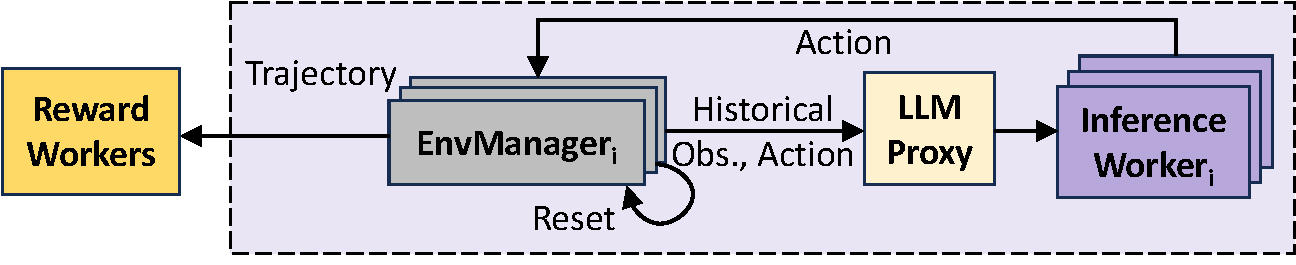
\includegraphics[width=\linewidth]{figs/overview/traj-level-rollout.pdf}
    \vspace{-10pt}
    \caption{Trajectory-Level Rollout Overview.}
    \label{fig:traj_rollout}
\end{figure}

\subsection{Asynchronous Workflows}
\label{subsec:async-workflow}
We describe the asynchronous workflows in \SystemName{} that realize fine-grained asynchrony (\textbf{Principle 2}). Within rollout, LLM generation is overlapped with environment execution. Across stages, rollout is overlapped with reward and training.

\PHM{\texttt{LLMProxy}: Trajectory-Level LLM Generation.} \texttt{LLMProxy} is a gateway that decouples LLM serving clients from the underlying serving instances. It intelligently orchestrates requests across a fleet of internal LLM inference workers. Each worker is built around a command-driven event loop that manages an inference engine (e.g., vLLM~\cite{vllm}, SGLang~\cite{sglang}).

This loop runs continuously in a non-blocking fashion with two components:  
(1) \textit{Step-wise command processing.} The loop continuously polls for commands dispatched from \texttt{LLMProxy}, \texttt{ADD} to enqueue new requests and \texttt{ABORT} to cancel existing ones. When no commands are pending, it advances the inference engine by executing a single decode or prefill step for a batch of requests, keeping GPU utilization high. This design ensures that adding or aborting an ongoing trajectory does not stall the entire LLM generation process.  (2) \textit{Post-processing.} When the LLM engine finishes a request after a certain prefill/decoding step, the loop immediately invokes a pre-registered callback. This callback post-processes the output and returns the result to the original client (e.g., an \texttt{EnvManager}). This allows each trajectory to perform environment interaction as soon as its LLM generation completes, without waiting for stragglers. Together, both functions enable trajectory-level LLM generation. 




\PHM{\texttt{EnvManager}: Trajectory-level Environment Interaction.} Each \texttt{EnvManager} is a lightweight controller that manages the lifecycle of a single environment to collect trajectories, as shown in \autoref{fig:traj_rollout}. It begins with environment initialization via \texttt{reset}, after which it enters an independent event loop that orchestrates the interaction between an environment instance and the shared \texttt{LLMProxy}. During this loop, the \texttt{EnvManager} maintains a list of (observation, action) pairs to construct a trajectory. Specifically, it feeds \texttt{LLMProxy} with the historical (observation, action) sequence as input to obtain the next action, applies this action to the environment via \texttt{step}, and records the resulting observation. % This loop repeats until a termination criterion is met. 

In practice, \SystemName{} launches multiple \texttt{EnvManager} instances simultaneously, and each \texttt{EnvManager} yields a single trajectory rather than batch-executing environment interactions (as shown in \autoref{fig:sub-batched_env_interaction}). As a result, long-tail environment workers do not delay the execution of other workers. Combined with trajectory-level LLM generation, \SystemName{} can overlap LLM generation with environment interaction in a fine-grained manner. Furthermore, upon completing a trajectory, the \texttt{EnvManager} immediately invokes a reward computation function via a serverless API as a non-blocking task, allowing reward computation to overlap with ongoing rollouts. Overall, this trajectory-level rollout management enables a high degree of parallelism to maximize throughput. 


\begin{figure}
    \centering
    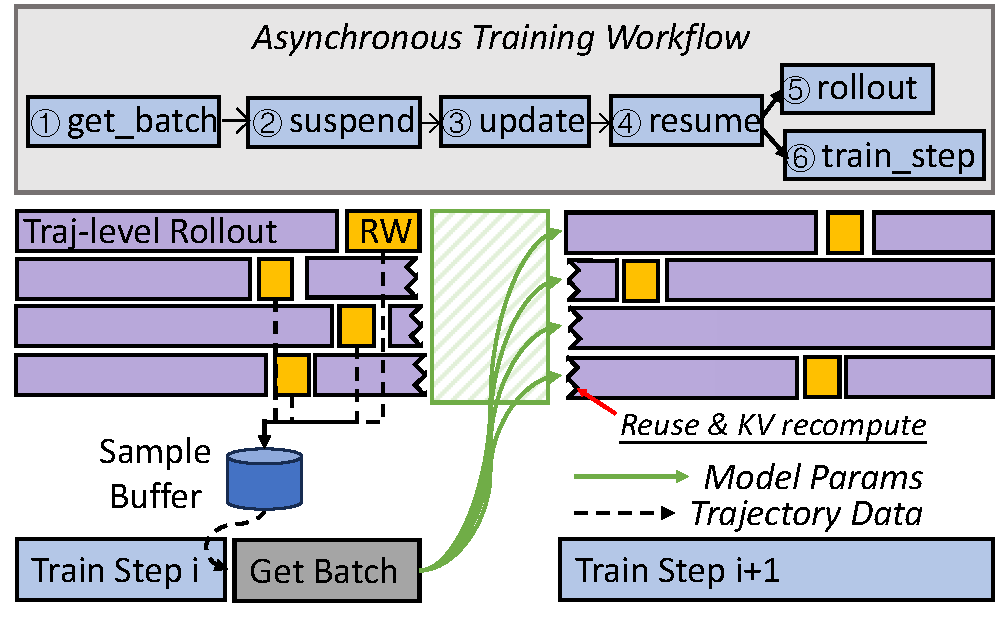
\includegraphics[width=0.9\linewidth]{figs/overview/rollout_scheduler_osdi_resume.pdf}
    % \vspace{-10pt}
    \caption{Asynchronous Training Workflow.}
    \label{fig:rollout_scheduler}
\end{figure}

\noindent\textit{\underline{Optimization: Redundant Env Rollouts.}}  
The trajectory-level design of \texttt{LLMProxy} and \texttt{EnvManager} enables an optimization we term \textit{redundant environment rollouts}. This technique allows users to launch more environments than strictly required to interact with the agent LLM. Once the target number of trajectories has been collected, any ongoing rollouts can be terminated and even aborted. Because rollouts are managed at the trajectory level, slow environments do not block or delay faster ones. This effectively mitigates fail-slow and fail-stop environments. 
Our empirical analysis in \S\ref{subsec:eval-async} reveals that this technique improves rollout efficiency.
Furthermore, large-scale deployments in \S\ref{sec:large-scale-analysis} benefit from this by avoiding the impact of environment failures.


\PHM{Asynchronous Training Workflow.}
\autoref{fig:rollout_scheduler} shows how \SystemName{} orchestrates the asynchronous training workflow. In the rollout stage, multiple \texttt{EnvManager}s act independently, continuously 
% interacting with \texttt{LLMProxy} to generate 
generating trajectories and enqueue them into the \texttt{SampleBuffer}. LLM inference and training workers run on separate GPUs, enabling disaggregated training.

The training workflow periodically runs a weight synchronization protocol. It first invokes a blocking \texttt{get\_batch} call to retrieve a batch of trajectories from the \texttt{SampleBuffer}. It then issues a \texttt{suspend} command to halt trajectory collection, performs a \texttt{model\_update} by fetching the latest LLM and broadcasting its weights to all inference workers.
This process is accelerated by the non-blocking, cross-cluster communication optimization detailed in \S\ref{sec:cluster}.
Subsequently, it issues a \texttt{resume} command to continue the trajectory-level rollout with the updated model.
\emph{Unfinished trajectories from the previous iteration are also reused in the current one, through 
KV cache recomputation}. Last, it executes \texttt{train\_step} on the retrieved data. In asynchronous training mode, the training stage overlaps with the rollout stage, and \SystemName{} controls the staleness of a trajectory with asynchronous bound.


\PHM{Asynchronous Bound.}
In asynchronous training, trajectory generation can be interrupted and later resumed under a newer agent LLM. Thus, a single batch of trajectories may be generated by multiple versions of LLM. The staleness introduces high variance and compromise training stability. AReaL~\cite{areal} addresses this by constraining the average sample freshness within each batch to preserve model quality. Differently, \SystemName{} introduces an \textbf{asynchronous bound} $\alpha$ to regulate freshness at the per-trajectory level and to actively manage the asynchronous workflow. It is defined per trajectory as the maximum allowable gap in version numbers between the current agent LLM and the version that initiated generation of that trajectory. If the agent LLM has advanced to version $n$, then any trajectory in \texttt{SampleBuffer} must have been initiated by a version no older than $(n - \alpha)$. Trajectories that violate this constraint are aborted. Our empirical study (\S\ref{ssec:e2e-performance}) suggests that setting the asynchronous bound to one yields a balance between training speed and stability.


%!TEX root=../main.tex
\section{System Architecture}
\label{sec:architecture}
\begin{figure}
    \centering
    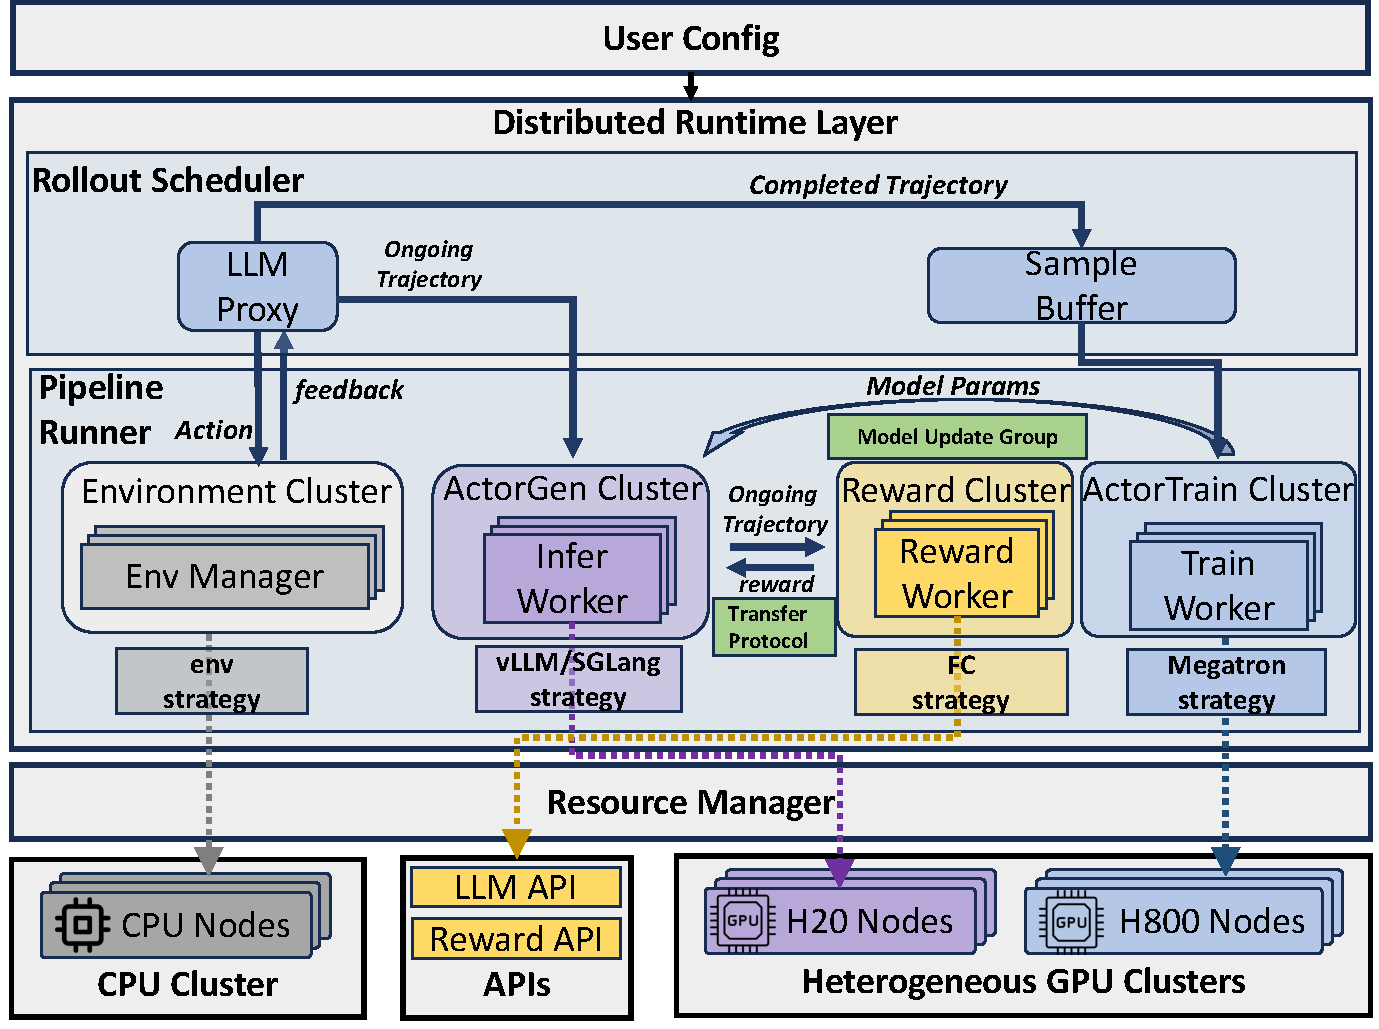
\includegraphics[width=0.9\linewidth]{figs/overview/sys_arch_osdi_updated.pdf}
    \caption{System Architecture of \SystemName{}}
    \label{fig:sys_arch}
\end{figure}


We implemented \SystemName{} in approximately 60k lines of Python code. 
\autoref{fig:sys_arch} shows the architecture of \SystemName{} consisting of the distributed runtime layer and the resource manager.
\SystemName{} parses user configurations and constructs the training pipeline atop the distributed runtime. The runtime includes a rollout scheduler that manages the rollout execution workflow and the \texttt{Cluster} runtime that performs distributed computation and communication. The resource manager allocates heterogeneous resources from a shared  pool to the workers.

\noindent\textbf{Rollout Scheduler.} It controls the rollout stage via managing the lifecycle of each trajectory. The \texttt{LLMProxy} interacts with multiple environment managers and routes ongoing trajectories to appropriate inference workers. Completed trajectories are added to \texttt{SampleBuffer} for subsequent model training. 


\noindent\textbf{Pipeline Runner.} The pipeline runner consists of multiple \texttt{Cluster}s that assume different roles in agentic RL training (e.g., reward, environment). Each \texttt{Cluster} orchestrates a collection of workers to perform a specific type of distributed computation (e.g., training, generation, environment interaction) using a chosen strategy (e.g., vLLM~\cite{vllm}, Megatron~\cite{shoeybi2019megatron}, Function Compute~\cite{alibaba_function_compute}). 
% \texttt{Cluster}s exchange trajectories via a transfer protocol, with trajectories represented as \texttt{ObjRef} objects provided by Ray~\cite{ray}, enabling deferred object materialization and hiding data transmission overhead.
\texttt{Cluster}s exchange trajectories via Ray's \texttt{ObjRef}s~\cite{ray}, which enables deferred materialization and hides data transmission overhead by passing object references instead of data copies.
For model weight synchronization, each \texttt{Cluster} exposes a \texttt{model\_update\_group} interface that leverages high‑throughput transfer engines such as NCCL~\cite{nccl} and Mooncake~\cite{qin2024mooncake}, utilizing NVLink, InfiniBand, and Ethernet to efficiently synchronize weights.

\noindent\textbf{Resource Manager.} The resource manager uses a persistent metadata store to maintain a real-time view of critical state, including the distributed runtime state, cluster resource availability, and service API availability. When it receives a worker deployment request, it first consults the metadata store to validate the request, then binds the requested resources or external services to the workers.


% \input{contents/5implementation}
%!TEX root=../main.tex
\section{Performance Evaluation}
\label{sec:eval}

In this section, we present the end-to-end evaluation (\S\ref{ssec:e2e-performance}) and the analysis of three design principles (\S\ref{subsec:eval-disaggregated}–\ref{subsec:eval-reward-worker}). 

\begin{figure*}[tb]
    \centering
    \begin{subfigure}[b]{0.466\linewidth}
        \centering
        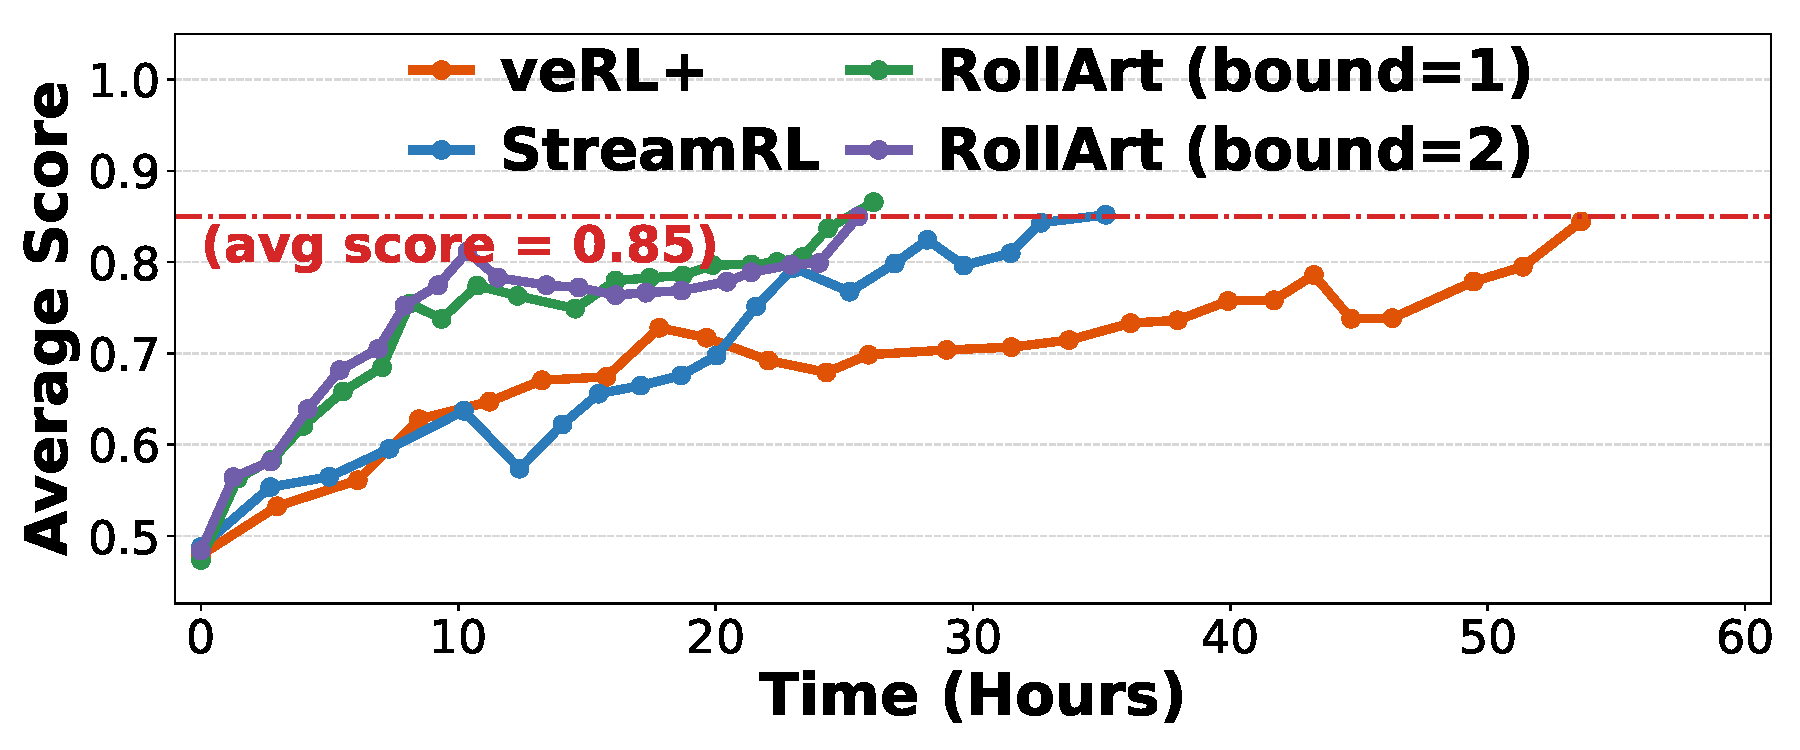
\includegraphics[width=\linewidth]{figs/e2e/score_comparison.pdf}
        \caption{Time-to-score.}
        \label{fig:e2e-acc}
    \end{subfigure}
    \begin{subfigure}[b]{0.31\linewidth}
        \centering
        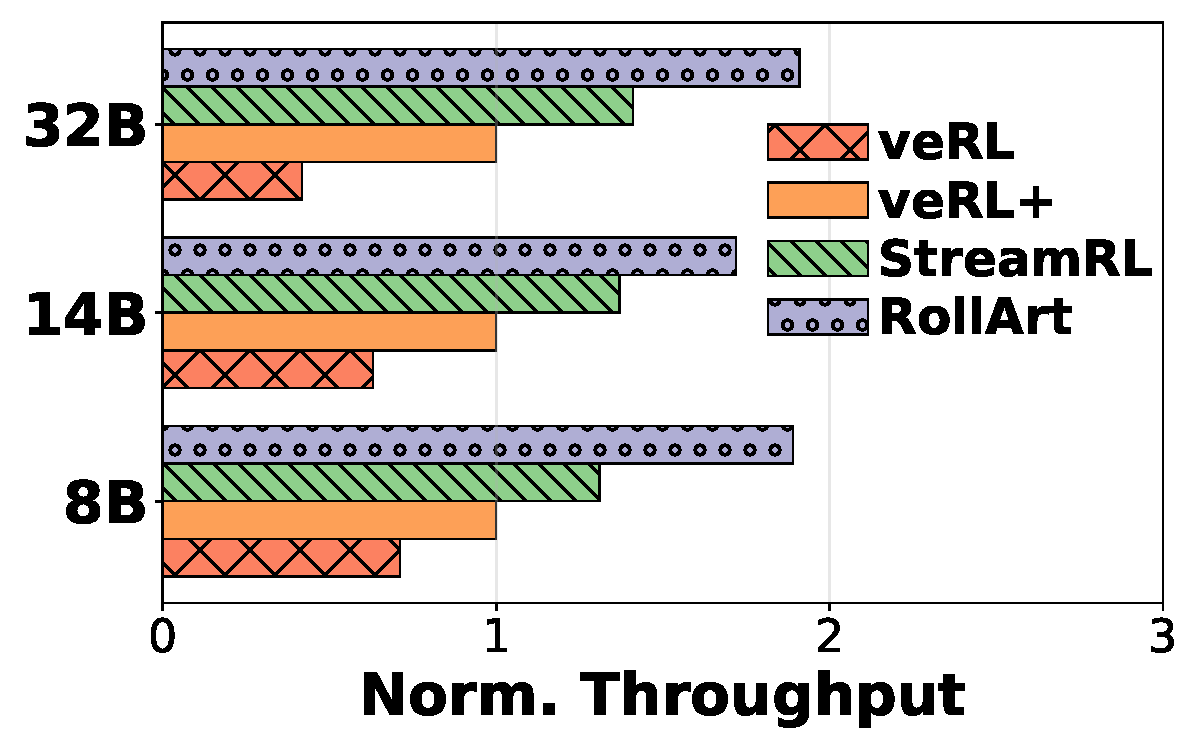
\includegraphics[width=\linewidth]{figs/e2e/modelsize_thr_horizontal.pdf}
        \caption{Throughput Efficiency.}
        \label{fig:e2e-thr}
    \end{subfigure}
    \begin{subfigure}[b]{0.214\linewidth}
        \centering
        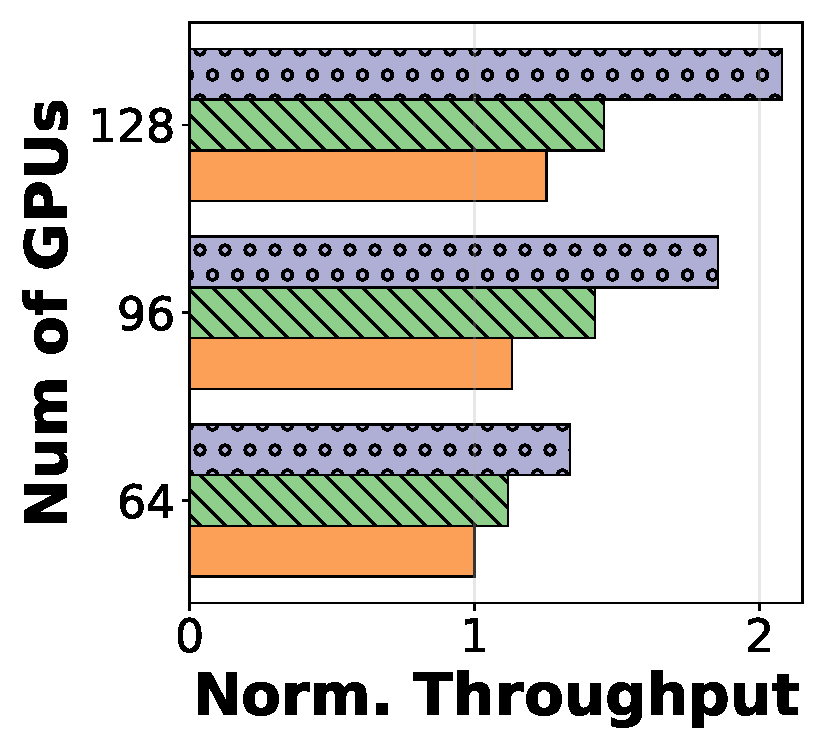
\includegraphics[width=\linewidth]{figs/e2e/modelsize_scaling_horizontal.pdf}
        \caption{Resource Scaling.}
        \label{fig:e2e-thr-scaling}
    \end{subfigure}


    \caption{
        Comparison of (a) end-to-end time-to-score on Qwen3-32B;
        (b) normalized throughput across LLMs for different approaches; and (c) normalized throughput of Qwen3-14B across different numbers of H800 GPUs.
    }
    \label{fig:e2e-combined}
    \vspace{-10pt}
\end{figure*}


\subsection{Evaluation Setup}

\noindent\textbf{Models and Tasks.} 
We train Qwen3~\cite{yang2025qwen3technicalreport} LLM family (8B–32B) on a diverse mixture of agentic tasks (\autoref{tab:env-taxomy}). All models are configured with a maximum context length of 32K tokens. Due to the difficulty of the \texttt{SWE-bench} agentic task, we train it only on Qwen3-32B. we employ a 7B reward LLM to validate the reasoning process of mathematical task. 


\noindent\textbf{Training Configurations.} We use the GRPO algorithm~\cite{he2025deepmath} with a training batch size of 512, a group size of 8, and a uniform sampling ratio across all tasks. For asynchronous training, we allocate 32 H800 GPUs to the training stage and use the remaining H20 and H800 GPUs for rollouts. During rollout, the tensor-parallelism degrees for Qwen3-8B/14B/32B are set to 1, 2, and 4, respectively, and we tune the training parallelism to maximize throughput. We run rollouts on vLLM 0.8.4 and training on Megatron v0.12.2, with prefix caching and CUDA graphs enabled during rollout.


\noindent\textbf{Weight Update Engine.} We use NCCL~\cite{nccl} v2.26.5 to perform intra-cluster weight update and Mooncake v0.3.7~\cite{qin2024mooncake} storage server for cross-cluster communication. 

\noindent\textbf{Hardwares.} \SystemName{} is deployed on an H800 cluster with 96 GPUs and an H20 cluster with 32 GPUs. Within each cluster, GPU nodes are connected via 400 Gbps InfiniBand, while cross-cluster communication uses a 200 Gbps Ethernet network. We use a dedicated CPU cluster for \texttt{SWE-bench} and another for the remaining environments. The reward workers run on our internal serverless platform. Without clarification, all experiments are performed with 128 GPUs. 

\noindent\textbf{Baselines.} Since no existing open-source system supports our full spectrum of agentic tasks, we follow the synchronous RL implementation of veRL (\textbf{veRL}). To strengthen this baseline, we additionally enable asynchronous reward computation, asynchronous environment interaction, and \textit{Reward-as-a-Service}, and denote this as \textbf{veRL+}. We also compare against StreamRL~\cite{StreamRL} and enable the one-off training paradigm~\cite{deepscaler2025} (see \autoref{fig:paradigm-all-in-one}-Left), which parallelizes rollout and training by consuming trajectories generated in the previous step. The optimizations used in veRL+ are also applied to StreamRL. We use Megatron~\cite{shoeybi2019megatron} for the training stage, which does not support heterogeneous GPU configurations. StreamRL likewise does not support heterogeneous GPUs during rollout. For simplicity, we run both baselines on 128 H800 GPUs; consequently, \SystemName{} incurs roughly 83\% of the baselines’ per-GPU-hour cost.

\noindent\textbf{Metrics.} We measure end-to-end latency as the average step time over five iterations. The throughput is the total number of prompt and response tokens in a global batch by the step time~\cite{sheng2025hybridflow}. We report average validation score across all tasks.



\subsection{End-to-End Evaluation}
\label{ssec:e2e-performance}


\noindent\textbf{Model Convergence.} We measure the score per ten iterations and report time-to-score with a target score of 0.85 in \autoref{fig:e2e-acc}. StreamRL achieves a 1.52\(\times\) end-to-end latency speedup over the veRL+ baseline by overlapping training and rollout. \SystemName{} keeps the rollout GPUs saturated by launching more rollouts and reusing partially generated trajectories across iterations. Consequently, with a bound of 1, the asynchronous approach delivers a 2.05\(\times\) and 1.35 \(\times\) step time reduction over the veRL+ and StreamRL. Although the asynchronous configuration with a bound of 2 exhibits a faster initial convergence rate, it results in a slightly worse time-to-score than the bound of one at later stages. Overall, different bounds still provide satisfactory convergence performance.

\noindent\textbf{Throughput Efficiency.} We present the throughput efficiency of different approaches in \autoref{fig:e2e-thr}. We normalize the throughput results to veRL+ baseline. We set the bound to 1 for \SystemName{}. The optimization techniques including asynchronous reward and envinvornment interaction as well as serverless reward worker can improve 1.40-2.40\(\times\) throughput. By overlapping rollout and training stage, we can see StreamRL achieves 1.31-1.47\(\times\) throughput increase. By fine-grained ascynrhony, \SystemName{} can provide 2.65-4.58\(\times\) throughput over the Sync baseline. Overall, \SystemName{} achieves substantial advantages in throughput efficiency.



\noindent\textbf{Resource Scaling.} We further evaluate the resource scaling performance of \SystemName{}. Specifically, we conduct experiments on 128 H800 GPUs and vary the number of GPUs allocated to rollout from 64 to 128 for different approaches. \autoref{fig:e2e-thr-scaling} reports the normalized throughput to veRL+ baseline running on 64 H800 GPUs. As the number of allocated GPUs increases, the marginal throughput gains diminish for veRL+ and StreamRL. However, the asynchronous RL training in \SystemName{} continues to yield 1.33-2.08\(\times\) throughput improvements, demonstrating superior resource scaling efficiency. 



\subsection{Analysis of Hardware Affinity}
\label{subsec:eval-disaggregated}

\begin{figure}[tb]
    \centering
    \begin{subfigure}{0.47\linewidth}
        \centering
        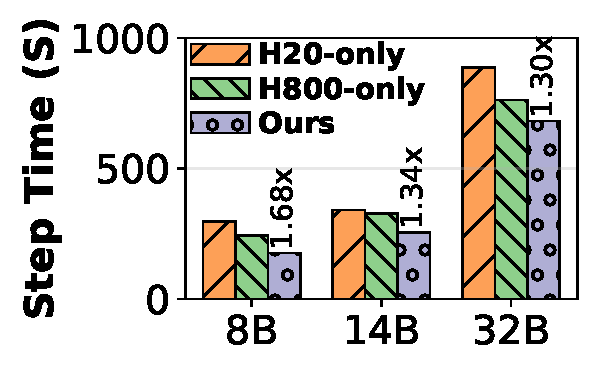
\includegraphics[width=\linewidth]{figs/col_dis/hw_affinity_3bars_small.pdf}
        \caption{Rollout Efficiency.}
        \label{fig:compute-efficiency}
    \end{subfigure}
    \begin{subfigure}{0.47\linewidth}
        \centering
        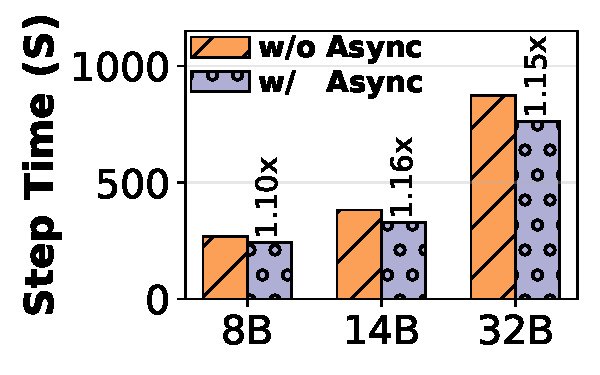
\includegraphics[width=\linewidth]{figs/col_dis/synctime.pdf}
        \caption{Cross-Cluster Comm.}
        \label{fig:comm-efficiency}
    \end{subfigure}
    % \vspace{-10pt}
    \caption{ \textbf{[Principle 1]}: (a) The efficiency of hardware affinity; (b) The benefit of async cross-cluster communication.}
    \label{fig:rollout_col_disagg}
    % \vspace{-10pt}
\end{figure}

% Rollout time for running different LLMs on a homogeneous H20 cluster, a homogeneous H800 cluster, and a heterogeneous cluster.

\noindent\textbf{Training Efficiency.} We evaluate the training efficiency on compute-optimized and bandwidth-optimized hardware across LLMs. To isolate the impact of hardware affinity, we fix the training allocation to 32 H800 GPUs and use three resource configurations for rollout: 72 H800 GPUs as the H800-only baseline, 208 H20 GPUs as the H20-only baseline, and an affinity-aware setting with 64 H800 GPUs plus 24 H20 GPUs. In the affinity-aware setup, mathematical and game-oriented agentic tasks are prioritized routed to H20 GPUs. As shown in \autoref{fig:compute-efficiency}, \SystemName{} achieves a 1.30–1.68\(\times\) step time speedup across LLM sizes compared to H20-only configuration and 1.12-1.37 speedup compared to H800-only configuration due to more H20 GPU scan reduce resource contention and benefit to decoding heavy tasks. The H20-only configuration performs worst, suggesting that many agentic tasks benefit more from compute-optimized GPUs due to frequent prefill operations. Overall, exploiting the complementary strengths of heterogeneous hardware for rollout is crucial for improving training efficiency.


\noindent\textbf{Async Cross-cluster Communication.} Hardware affinity introduces cross-cluster weight update, where Ethernet-connected clusters incur high communication overhead. In contrast to veRL’s NCCL-based communication, which assumes that all GPU servers are connected with uniformly high-bandwidth links, our setting must explicitly handle heterogeneous interconnects. \autoref{fig:comm-efficiency} compares the end-to-end step time of our asynchronous cross-cluster communication with veRL’s approach. The asynchronous communication technique achieves a 1.10-1.16\(\times\) reduction in end-to-end step time across LLMs, indicating that cross-cluster communication overhead deserves dedicated optimization.


% Here, we evaluate how asynchronous cross-cluster communication can hide the heavy cross-clsuter weight transfer. To emphasize the gains of this technique, we 

% ethernet

% \SystemName{} introduce asynchronous cross-cluster communication to prevent the low-bandwidht links a

% We evaluate our cross-cluster communication optimizations against veRL’s NCCL-based cross-cluster communication as the baseline. Specifically, we train Qwen3-8B on a rollout cluster with 8 H800 and H20 GPUs connected via 200 Gbps TCP, using a batch size of 32. \autoref{fig:comm-efficiency} reports the end-to-end step time. We observe that the optimized cross-cluster communication achieves a 1.10–1.16\(\times\) reduction in end-to-end latency across different LLMs, confirming its effectiveness.



\begin{figure}[tb]
    \centering
    \begin{subfigure}{0.23\textwidth}
        \centering
        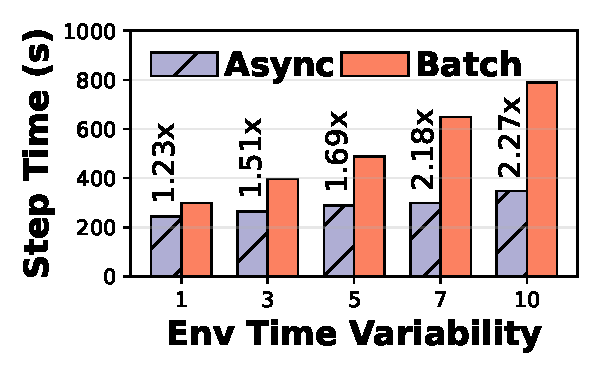
\includegraphics[width=\linewidth]{figs/async_env/async_env_time_var_bar.pdf}
        \caption{Env Time Variability.}
        \label{subfig:async_env_batch}
    \end{subfigure}
    \begin{subfigure}{0.23\textwidth}
        \centering
        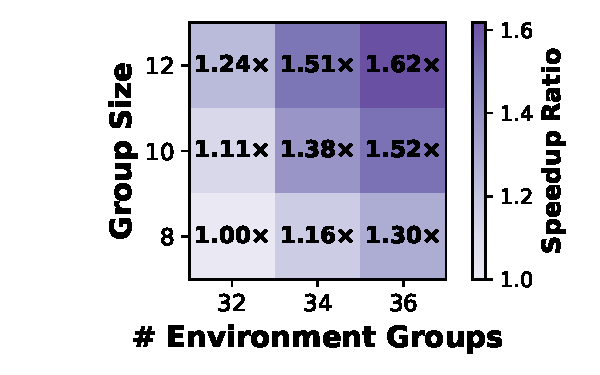
\includegraphics[width=\linewidth]{figs/async_env/async_env_redunant.pdf}
        \caption{Redundant Env Rollout.}
        \label{subfig:env-red-rollout}
    \end{subfigure}
    \vspace{-5pt}
    \caption{\textbf{[Principle 2]}: Benefits of trajectory-level Env.}
    \label{fig:rollout_env_async}
    % \vspace{-10pt}
\end{figure}




\begin{figure}[tb]
    \centering
    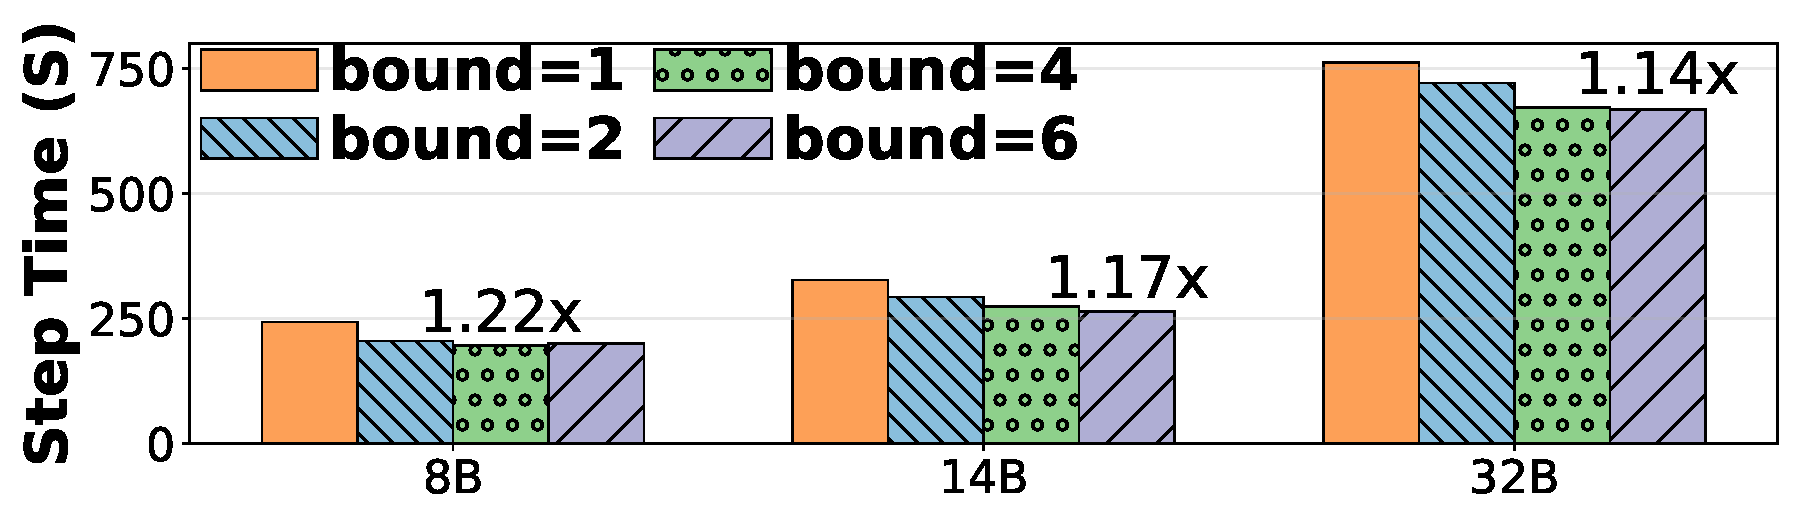
\includegraphics[width=0.9\linewidth]{figs/async_train/async_ratio.pdf}
    \vspace{-5pt}
    \caption{\textbf{[Principle 2]}: The average step time comparison of different asynchronous bounds across LLMs.}
    \label{fig:async-ratio}
\end{figure}


\subsection{Analysis of Trajectory-level Asynchrony}
\label{subsec:eval-async}
\noindent\textbf{Asynchronous Environment Interaction.} Trajectory-level environment management enables asynchronous environment interaction. We run Qwen3-8B/32K and inject additional environment latency sampled from gaussian distributions with mean \(\mu = 10\) and standard deviation \(\sigma\) ranging from 1 to 10 at each turn. We compare trajectory-level and batch-level interaction in \autoref{subfig:async_env_batch}, reporting the average step time over ten iterations. As the latency variance increases, the performance gains of trajectory-level over batch-level interaction grows from \(1.23\times\) to \(2.27\times\), proving asynchronous environment interaction sustains high throughput.

\noindent\textbf{Redundant Environment Rollouts.} GRPO exposes two key configuration parameters: the number of environment groups and the group size. By launching additional environments, redundant rollouts can tolerate environment failures and accelerate training. We run Qwen3-8B/32K on 32 H800 GPUs and vary both the number of environment groups and the group size on the \texttt{GEM-math} agentic task, reporting rollout speedup ratios in \autoref{subfig:env-red-rollout}. The maximum speedup reaches \(1.62\times\), and increasing either parameter yields positive speedup.

\noindent\textbf{Impact of Asynchrony Bound.}
We vary the asynchronous bound from 1 to 6 and report the average step time across LLMs in \autoref{fig:async-ratio}. Increasing the bound typically reduces the probability of aborting completed trajectories due to staleness, which in turn lowers the step time in most cases. However, we observe that efficiency plateaus within certain ranges. The optimal bound differs across LLMs and yields at most a 1.22\(\times\) step time reduction compared with a bound of 1. Considering overall training performance, these throughput gains do not necessarily translate into better time-to-score. In practice, setting the bound to one delivers satisfactory performance.

\begin{figure}[tb]
    \centering
    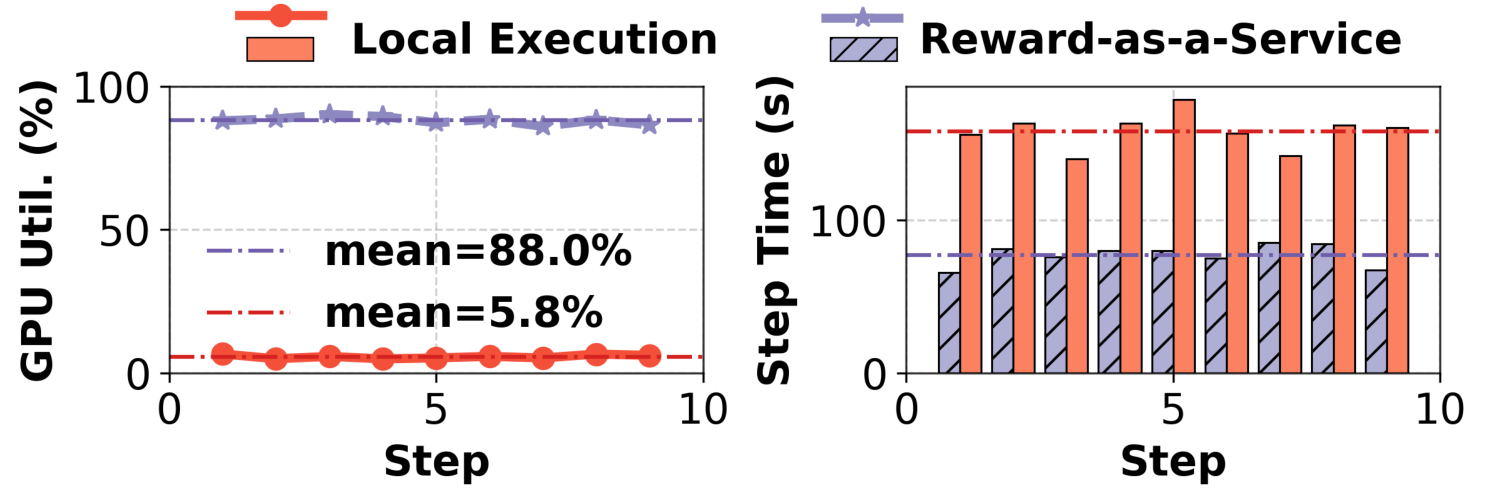
\includegraphics[width=\linewidth]{figs/reward/7B_experiments_comparison.pdf}
    \vspace{-15pt}
    \caption{\textbf{[Principle 3]}: Comparison between dedicating local GPUs and using Reward-as-a-Service.}
    \label{fig:reward_comparison_exp}
    % \vspace{-5mm}
\end{figure}

\begin{figure*}[tb]
    \centering
    \begin{subfigure}[b]{0.33\linewidth}
        \centering
        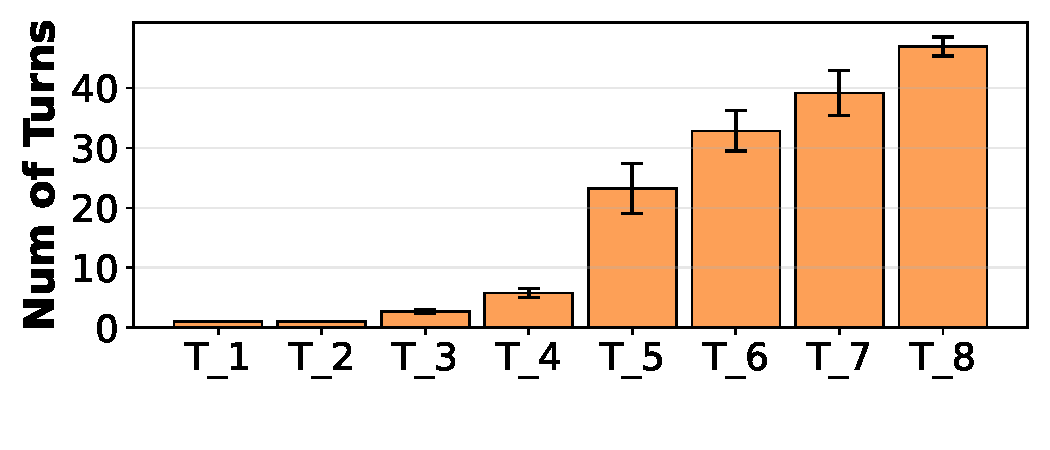
\includegraphics[width=\linewidth]{figs/trace/action.pdf}
        \caption{Average Number of Turns per Task.}
        \label{fig:action}
    \end{subfigure}
    % \hfill
    \begin{subfigure}[b]{0.33\linewidth}
        \centering
        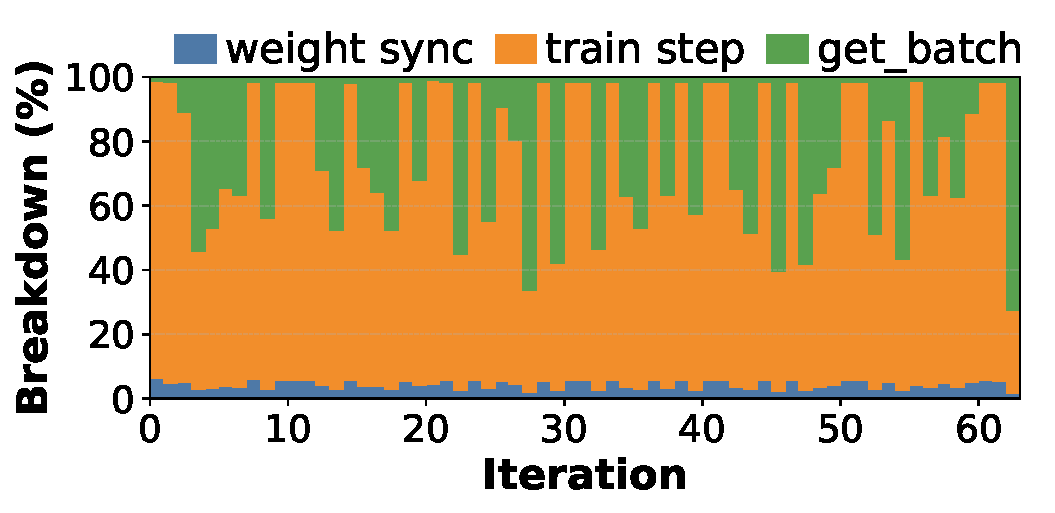
\includegraphics[width=\linewidth]{figs/trace/trace_dist.pdf}
        \caption{Step Time Distribution.}
        \label{fig:trace_dist}
    \end{subfigure}
    \begin{subfigure}[b]{0.33\linewidth}
        \centering
        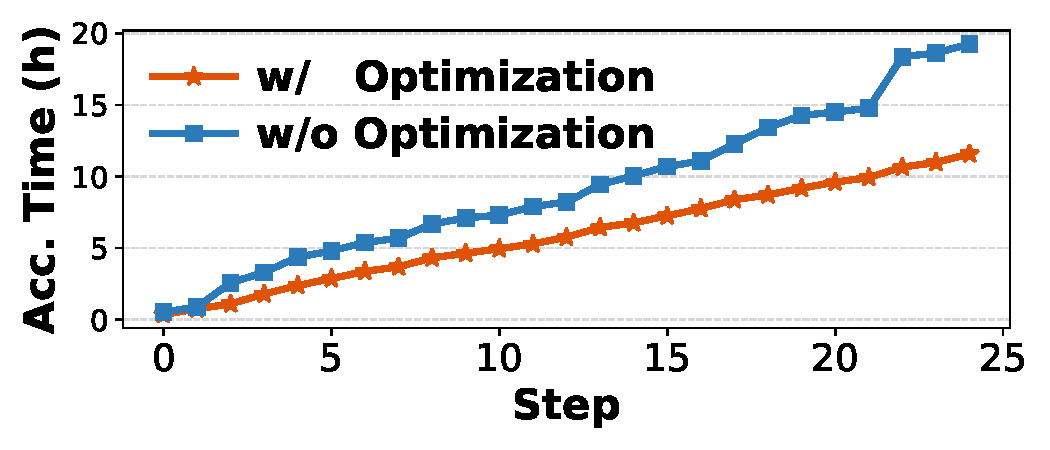
\includegraphics[width=\linewidth]{figs/trace/total_iter_time.pdf}
        \caption{Accumulated Step Time.}
        \label{fig:opt_step_time}
    \end{subfigure}
    \caption{Production-Grade Agentic RL Workload Characterization.}
    \vspace{-10pt}
    \label{fig:workload_overview}
\end{figure*}

\subsection{Benefits of Serverless Reward Worker}
\label{subsec:eval-reward-worker}
We evaluate \textit{Reward-as-a-Service} by comparing it with a dedicated local GPU setup. We run three concurrent agentic RL jobs on mathematical tasks with Qwen3-8B/16K as the agent and Qwen2.5-7B as the reward LLM on a 16-GPU cluster, using eight GPUs for training. In the local setup, four GPUs are reserved for the reward LLM. \autoref{fig:reward_comparison_exp} shows GPU utilization and rollout time per step for a batch size of 84, where rollout time includes asynchronous reward computation. The serverless platform is shared by three jobs and perform autoscaling, increasing average GPU utilization from 6\% to 88\%. Without the hot-standby GPUs for reward computation, more GPUs can be utilized for rollouts. Thus, the average rollout time reduces from 158 seconds to 77 seconds, demonstrating the benefits of statefulness-aware computation.

%!TEX root=../main.tex

\section{\SystemName{} in Production}
\label{sec:large-scale-analysis}



Over the past six months, thousands of agentic RL jobs have used \SystemName{} for post-training. 
To further demonstrate its scalability and robustness, we share our
experience on a large production cluster with more than 3,000 GPUs. 




\PHM{Workload Characterization}
We trained an MoE LLM (hundreds of billions of parameters) using \SystemName{} over in-house datasets for agentic tasks like mathematics and software engineering. 
The maximum prompt length and response length are 12k and 46k respectively. 
The average number of turns per task varies from one to 48 (\autoref{fig:action}), confirming the coexistence of joint prefill-heavy and decode-heavy tasks in agentic RL training. 
\emph{The large number of turns requires a highly stable environment and fast prefill computation.}



This job adopts asynchronous training with a 1:5 ratio of training to generation GPUs. 
To balance gradient stability and rollout efficiency, an asynchronous bound of one is used, leading to maximum iteration time of 1.5 hours (see \autoref{fig:trace_dist} for iteration time distributions). 
The primary bottleneck is the blocking \texttt{get\_batch} call, after the training stage finishes computing log probabilities and gradients.
It waits for enough trajectories in \texttt{SampleBuffer} to reach the batch size. 
This consumes up to 62\% of the iteration time with GPU idleness, and eliminating it could ideally reduce end-to-end training time by 22\% (\autoref{fig:trace_dist}). \emph{The training stage may stall due to insufficient trajectories from the rollout stage, making it necessary to balance the throughput of both stages.}



\PHM{Characterization-driven Optimization.} 
Informed by the workload characterization, we adjust the resource allocation ratio and optimize the prefix caching for the MoE architecture. \autoref{fig:opt_step_time} shows that the characterization-drive optimization achieves 1.66$\times$ end-to-end speedup over the first 25 steps. Beyond this, we also provide dedicated optimizations for environments and system resilience. 



\PHM{Optimizing Environment Stability.} 
Operating thousands of concurrent, Docker-based agentic environments on Kubernetes necessitates critical optimizations to ensure stability and performance. 
To combat network instability and pull overhead in \texttt{env.reset}, we employ a multi-tiered caching architecture. The first tier consists of an internal image registry that acts as a local mirror, eliminating external network calls. A second-tier, distributed load-balanced cache is situated between the compute nodes and this registry to efficiently manage high-volume requests.
During an \texttt{env.reset} operation, clients prioritize fetching the required Docker image from this cache. This approach dramatically enhances the robustness of environment setup, producing above 99.99\% success rate for \texttt{env.reset}.



\noindent\textbf{System Resilience.} 
We enhance system resilience at both the network and system levels. To reduce timeouts when connecting to environments, we use a persistent session-based protocol instead of a request-based one and adopt a exponential backoff retries to handle temporary network issues. Our disaggregated architecture isolates failures so that a problem in one environment, reward, or inference worker does not affect the others. Kubernetes manages environment workers, and the serverless platform manages reward workers. When an inference worker fails, it is first restarted on the same GPU. If it fails again, it is removed, and its trajectories, stored in the storage engine, are resumed on healthy workers. If a training worker fails, we restart from the latest checkpoint. This design has proven highly robust, with only a single failure observed during a week-long training run.





%!TEX root=../main.tex
\section{Related Work}
\label{sec:related_works}


\PHB{RL Post-Training Systems.}
%说一下现在的一些post-RL training systems 
Many systems address the systems challenges of RL post-training. Early frameworks~\cite{Harper_NeMo_a_toolkit,deepspeedchat,hu2024openrlhf} adopt static, stage-specific GPU partitions, which lowers overall utilization when the workload balance shifts across stages. veRL~\cite{verl} instead uses a hybrid controller that co-locates multiple stages on the same GPUs to improve hardware efficiency. Subsequent systems~\cite{liu2025specrlacceleratingonpolicyreinforcement,chen2025respecoptimizingspeculativedecoding,cheng2025fastllmposttrainingdecoupled,shao2025beatlongtaildistributionaware,RhymeRL,zhong2024rlhfuseefficientrlhftraining,areal,asyncflow,Laminar,StreamRL} explore a range of acceleration techniques, including speculative decoding, fusion of pipeline stages to reduce orchestration overhead, asynchronous or decoupled training to hide latency, and various forms of resource disaggregation. \SystemName{} builds on the disaggregated and asynchronous paradigm and assigns workloads based on hardware affinity.



\PHM{Resource Disaggregation.} The concept of resource disaggregation, first proposed in early architectural work on memory~\cite{disaggregated-mem-isca09}, has become a cornerstone of modern system design. Recent systems like LegoOS~\cite{shan2018legoos} and Mira~\cite{guo2023mira} decouple hardware into separate resource pools that can be managed independently to improve utilization. This pattern is prevalent in LLM serving, where systems commonly disaggregate the prefill and decoding phases~\cite{distserve, patel2023splitwise, hu2024inference, strati2024dejavu, qin2024mooncake}, with some even disaggregating transformer sub-modules like attention and FFNs~\cite{megascale-infer,step3}. In the context of RL post-training, several works apply a similar principle, separating the training and rollout stages across different GPU types~\cite{StreamRL,seamlessflow}. Compared to these approaches, \SystemName{} provides a more general and fine-grained disaggregation model, tailored specifically for the entire lifecycle of multi-task agentic RL. 




\section{Conclusion}
In this paper, we design an efficient and scalable disaggregated RL training system. We introduce its programming model, computation model, and system architecture, all guided by three core design principles. Our microbenchmarks and macrobenchmarks demonstrate that \SystemName{} delivers substantial improvements in resource efficiency, scalability, and system resilience in production-level clusters. 



% \clearpage

\bibliographystyle{plain}
\bibliography{reference}
\end{document}


Agentic Reinforcement Learning (RL) enables Large Language Models (LLMs) to perform autonomous decision-making and long-term planning. Unlike standard LLM post-training, agentic RL workloads are highly heterogeneous, combining compute-intensive prefill phases, bandwidth-bound decoding, and stateful, CPU-heavy environment simulations. We argue that efficient agentic RL training requires disaggregated infrastructure to leverage specialized, best-fit hardware. However, naive disaggregation introduces substantial synchronization overhead and resource underutilization due to the complex dependencies between stages.

We present RollArc, a distributed system designed to maximize throughput for multi-task agentic RL on disaggregated infrastructure. RollArc is built on three core principles: (1) hardware-affinity workload mapping, which routes compute-bound and bandwidth-bound tasks to bestfit GPU devices, (2) fine-grained asynchrony, which manages execution at the trajectory level to mitigate resource bubbles, and (3) statefulness-aware computation, which offloads stateless components (e.g., reward models) to serverless infrastructure for elastic scaling. Our results demonstrate that RollArc effectively improves training throughput and achieves 1.35-2.05\(\times\) end-to-end training time reduction compared to monolithic and synchronous baselines. We also evaluate RollArc by training a hundreds-of-billions-parameter MoE model for Qoder product on an Alibaba cluster with more than 3,000 GPUs, further demonstrating RollArc scalability and robustness. The code is available at https://github.com/alibaba/ROLL.